\documentclass{article}
\usepackage[english]{babel}
\usepackage{geometry,amsmath,amssymb,graphicx,alltt}
\geometry{b4paper, paperheight= auto, paperwidth= auto}

%%%%%%%%%% Start TeXmacs macros
\catcode`\>=\active \def>{
\fontencoding{T1}\selectfont\symbol{62}\fontencoding{\encodingdefault}}
\newcommand{\nobracket}{}
\newcommand{\nocomma}{}
\newcommand{\tmaffiliation}[1]{\\ #1}
\newcommand{\tmop}[1]{\ensuremath{\operatorname{#1}}}
\newcommand{\tmrsub}[1]{\ensuremath{_{\textrm{#1}}}}
\newcommand{\tmstrong}[1]{\textbf{#1}}
\newcommand{\tmtextit}[1]{{\itshape{#1}}}
\newcommand{\tmtexttt}[1]{{\ttfamily{#1}}}
\newenvironment{tmcode}[1][]{\begin{alltt} }{\end{alltt}}
%%%%%%%%%% End TeXmacs macros

\begin{document}

\title{Particle In Cell (PIC) simulation}

\author{
  Youjun Hu
  \tmaffiliation{Email: yjhu@ipp.cas.cn\\
  Institute of Plasma Physics, Chinese Academy of Sciences}
}

\maketitle

\begin{abstract}
  This note reviews the basic theory of Particle-In-Cell (PIC) simulation of
  plasmas.
\end{abstract}

\

\section{Particle methods}

There are a class of numerical methods that make use of the characteristic
lines of hyperbolic Partial Differential Equations (PDEs). These methods
reduce a hyperbolic PDE to a family of ordinary differential equations that
can be integrated from initial values to get the the solution of the original
partial differential equation. By using the integration along the
characteristic lines, all partial derivatives of the unknown distribution
function with respect to phase-space coordinates are avoided, and thus this
method does not need a regular phase-space mesh to construct numerical
approximation to the phase-space partial differential operators. This enables
us to adopt random sampling of the phase-space, which has the advantage of
reducing the error in evaluating high-dimensional phase-space integration. In
this sense, this method can be considered as a kind of ``mesh-free'' method.

Since the characteristic lines are usually identical to the orbits of
particles/elements in the phase-space, these methods can be generally called
``particle methods''. In the core of particle methods, are the method of
characteristics and Monte-Carlo sampling and integration.

The computational nodes (often called markers/particles/super-particles) in
particle methods follow the particle orbits and thus their positions in
phase-space evolve with time, which is one of the differences between the
particle methods and the usual Euler-grid-based methods that usually uses
fixed grid-points. The evolving computational nodes in particle method are
often called Lagrangian markers while the fixed grids are often called Euler
grid-points. Therefore, particle method is a kind of {\tmstrong{mesh-free
Lagrangian}} method.

The so-called Particle-In-Cell (PIC) method, however, is a kind of
{\tmstrong{incomplete}} particle method, in which both evolving nodes
(mesh-free) and fixed grid-points (mesh) are used. Specificly, the kinetic
equation for the particle distribution function in the phase space is solved
by using mesh-free particle methods, whereas Maxwell's eqaution for the
electromagnetic field are solved by using spatial mesh. To obtain the source
terms in Maxwell's equation at grids, we need to calculate moments of the
distribution function represented by the mesh-free computational nodes. In PIC
simulations, the values of a moment at a spatial grid is approximated by the
averaged value of the moment in the corresponding spatial cell. This averaging
procedure, along with the use of finite spatial shape function of markers
(discussed later), has the effect of reducing (ideally removing) collisions
between particles. Collisions, if to be modeled, should be modeled by other
means.

For instance, in solving the Vlasov-Poisson equations by the PIC method, the
Vlasov equation for the phase-space distribution function is solved by using
the evolving nodes while the Poisson equation for the spatial electric
potential is solved by using the fixed grid-points. The special nomenclature
``particle-in-cell'' refers to the particular way of inferring the value of
charge density at the fixed spatial grid-points from the evolving coordinates
of computational markers. Therefore the PIC method is a kind of
{\tmstrong{hybrid particle-mesh methods}}.

\

This note discusses the basic theory of the Particle-In-Cell (PIC)
simulation, along with practical implementation in curvilinear coordinate
system. In the process of learning the PIC simulation method, I have developed
several toy Fortran codes to test what I have learned. The numerical results
given in these notes are obtained by using these codes. A copy of these codes
can be found at http://theory.ipp.ac.cn/\~{}yj/codes/pic\_1D\_src.tar

\subsection{Brief history of particle-mesh methods}

Particle-mesh (PM) method was invented in the 1950's at LANL for simulation of
compressible fluid flows. The first wide-spread application was for
collisionless plasma simulation, for which particle-mesh method was reinvented
in the 1960's and called particle in cell methods. These methods later also
obtained popularity in cosmology simulations.

\section{Phase-space sampling and markers' weight}

Particle simulations in space plasma physics community usually use the
Cartesian coordinate system, which is suitable for the simple configuration
considered there. In tokamak physics community, curvlinear coordinates are
usually used because of the toroidal configuration. (Another difference is
that the kinetic equation solved is usually the gyrokinetic one rather than
the primitive Vlasov equation.) Since my research interests are in tokamak
plasma, I will primarily use general curvilinear coordinate system in
presenting the PIC method. Specificly, the Jacobian of the coordinate system
will be explicitly shown in the formulas.

\subsection{Phase-space sampling and Phase space volume sampled by a marker}

Suppose the phase space $\mathbf{Z}= (\mathbf{r}, \mathbf{v})$ is described by
general curvlinear coordinates $(\alpha, \beta, \gamma, v_{\alpha}, v_{\beta},
v_{\gamma})$. Given a probability density function $P = P (\alpha, \beta,
\gamma, v_{\alpha}, v_{\beta}, v_{\gamma})$ that satisfies the following
normalization condition
\begin{equation}
  \label{18-9-20-p1} \int_{\Omega} P d V = 1,
\end{equation}
where $\Omega$ is the phase space region of interest, $d V$ is the phase-space
volume element. In terms of the $(\alpha, \beta, \gamma, v_{\alpha},
v_{\beta}, v_{\gamma})$ coordinates, $d V$ is given by $d V = | \mathcal{J}_r
\mathcal{J}_v | d \alpha d \beta d \gamma d v_{\alpha} d v_{\beta} d
v_{\gamma}$, where $\mathcal{J}_r$ is the Jacobian of transformation from
Cartesian space coordinates $(x, y, z)$ to curvlinear coordinates $(\alpha,
\beta, \gamma)$, and $\mathcal{J}_v$ is the Jacobian of transformation from
Cartesian velocity coordinates $(v_x, v_y, v_z)$ to curvlinear coordinates
$(v_{\alpha}, v_{\beta}, v_{\gamma})$. Using this, the normalization condition
(\ref{18-9-20-p1}) is written as
\begin{equation}
  \int_{\Omega} P | \mathcal{J}_r \mathcal{J}_v | d \alpha d \beta d \gamma d
  v_{\alpha} d v_{\beta} d v_{\gamma} = 1.
\end{equation}
Use this probability density function to sample the phase space region
$\Omega$ with $N$ markers, then the marker distribution function $g$ is given
by
\begin{equation}
  \label{18-10-27-p1} g = N \times P.
\end{equation}
The definition of $g$ implies that the number of markers within a small volume
of phase-space $d V$ is given by
\begin{equation}
  d N = g d V = g | \mathcal{J}_r \mathcal{J}_v | d \alpha d \beta d \gamma d
  v_{\alpha} d v_{\beta} d v_{\gamma} .
\end{equation}
Therefore the average phase space volume occupied (or sampled) by a marker,
$V_p$, is written as
\begin{equation}
  \label{16-3-22-p1} V_p \equiv \frac{d V}{d N} = \frac{1}{g} .
\end{equation}
In practical numerical implementation in a curvlinear coordinate system, I
prefer to define $P'$ and $g'$ by
\begin{equation}
  P' = P | \mathcal{J}_r \mathcal{J}_v |,
\end{equation}
and
\begin{equation}
  g' = g | \mathcal{J}_r \mathcal{J}_v |,
\end{equation}
where I explicitly include the coordinates transform Jacobian in the
definition of $P'$ and $g'$. Then equation (\ref{18-9-20-p1}) is written as
\begin{equation}
  \int_{\Omega} P' d \alpha d \beta d \gamma d v_{\alpha} d v_{\beta} d
  v_{\gamma} = 1,
\end{equation}
equation (\ref{18-10-27-p1}) is written as
\begin{equation}
  g' = N \times P',
\end{equation}
and the number of particle within the phase-space element $d \alpha d \beta d
\gamma d v_{\alpha} d v_{\beta} d v_{\gamma}$ is given by
\begin{equation}
  d N = g' d \alpha d \beta d \gamma d v_{\alpha} d v_{\beta} d v_{\gamma}
\end{equation}
i.e., $P'$ and $g'$ act respectively like a probability density function and
distribution function in terms of variables $(\alpha, \beta, \gamma,
v_{\alpha}, v_{\beta}, v_{\gamma})$ with the Jacobian equal to unity (i.e.,
$\alpha, \beta, \beta, v_{\alpha}, v_{\beta}, v_{\gamma}$ act as Cartesian
coordinates). The reason I do this is as follows. In many simulations, markers
are required to be loaded directly in $(\alpha, \beta, \gamma, v_{\alpha},
v_{\beta}, v_{\gamma})$ coordinates, i.e., these coordinates are directly
sampled. Then working in terms of $P'$ and $g'$ is more intuitive to me. In
terms of $g'$, the average phase space volume occupied by a marker is now
written as
\begin{equation}
  \label{18-1-28-p3} V_p = \frac{| \mathcal{J}_r \mathcal{J}_v |}{g'} .
\end{equation}
The methods of generating random numbers satisfying a given probability
density function are discussed in Sec. \ref{10-11-e1}.

If we use Cartesian coordinates $(x, y, z, v_x, v_y, v_z)$ to describe the
phase space, then it is obvious that $\mathcal{J}_r = 1$ and $\mathcal{J}_v =
1$.

\subsubsection{Time evolution of phase-space volume occupied by a marker}

Evaluate $V_p$ at the initial location of each marker and then assign this
value, $V_{p j 0}$, to the corresponding marker, i.e.,
\begin{equation}
  V_{p j 0} = \frac{1}{g (\mathbf{r}_{j 0}, \mathbf{v}_{j 0})} = \frac{|
  \mathcal{J}_r (\mathbf{r}_{j 0}) \mathcal{J}_v (\mathbf{r}_{j 0},
  \mathbf{v}_{j 0}) |}{g' (\mathbf{r}_{j 0}, \mathbf{v}_{j 0})},
\end{equation}
where $\mathbf{r}_{j 0}$ and $\mathbf{v}_{j 0}$ are the initial coordinates of
the $j \tmop{th}$ markers.

Further note that any particle distribution function $g$ in any
non-relativistic continuous electromagnetic field evolves as $d g / d t = 0$,
where $d / d t$ is the convective derivative in the phase space, i.e., the
distribution function is constant along a characteristic line. Since $V_p = 1
/ g$, it follows that,
\begin{equation}
  \frac{d}{d t} (V_{p j}) = 0,
\end{equation}
Therefore, $V_{p j}$ associated with a marker at later time is always equal to
the volume initially assigned to it, i.e., $V_{p j} = V_{p j 0}$. This is
assumed in most collisionless PIC simulation codes and related to the issue of
discrete particle noise. In practical simulation, we use finite number rather
than infinite number of markers to represent the marker distribution function
$g$. Due to this reason (the so-called discrete particle effect), $d
g_{\tmop{numerical}} / d t$ is never exactly zero. We can examine how accurate
$d g_{\tmop{numerical}} / d t \approx 0$ is by numerically count the number of
markers $\Delta N$ in a small phase volume $\Delta V$ around a marker and
examining the evolution of $\Delta N / \Delta V$. Some choices of the initial
state $g (\mathbf{x}, \mathbf{v}, t = 0)$ can make $d (\Delta N / \Delta V) /
d t$ smaller and thus reduce the noise introduced by the discrete particle
effect.

\subsection{Weights of markers}

Denote the physical particle distribution function in question by $f$ ($f$ can
be the full-f or $\delta f$, depending on the context). The weight of a marker
in this note is defined as the number of physical particles carried by $f$ in
the corresponding phase-space volume sampled by the marker, i.e.,
\begin{equation}
  w_j = f (\mathbf{Z}_j) d V_{p j},
\end{equation}
which, by using Eq. (\ref{16-3-22-p1}), \ is further written as
\begin{equation}
  \label{18-12-15-2} w_j = \frac{f (\mathbf{Z}_j)}{g (\mathbf{Z}_j)}
\end{equation}
or, by using Eq. (\ref{18-1-28-p3}), is written as
\begin{equation}
  w_j = \frac{f (\mathbf{Z}_j)}{g' (\mathbf{Z}_j)} | \mathcal{J}_r
  (\mathbf{Z}_j) \mathcal{J}_v (\mathbf{Z}_j) | .
\end{equation}

\subsubsection{Some discussions}

In most PIC codes I wrote, I implement several kinds of marker distribution
functions, which can be chosen via an option. In practice, I primarily use the
marker distribution $g$ that is uniform in real space and Maxwellian in
velocity space with a constant temperature (the other forms of marker
distributions are used occasionally for benchmarking purpose), i.e., $g$ is
given by
\begin{equation}
  \label{18-12-15-1} g = \frac{N_p}{V} \left( \frac{m}{2 \pi T_g} \right)^{3 /
  2} \exp \left( - \frac{m v^2}{2 T_g} \right),
\end{equation}
where $T_g$ is a constant temperature, $N_p$ is the number of markers, and $V$
is the spatial volume of the computational box. This marker distribution
satisfies the normalization $\int g d\mathbf{v}d\mathbf{r}= N_p$.

[In the literature on $\delta f$ PIC simulations, the weight defined by
different authors may differ by a factor and this factor is taken into account
when calculating velocity moments using the weight. For example, in Ben's
thesis{\cite{ben2016}}, the weight is defined as $w_{j \star} = \delta f /
f_0$, where $f_0$ is the equilibrium physical distribution function. Assume
that $f_0$ is an Maxwellian distribution with constant temperature $T_g$, then
the marker distribution given in Eq. (\ref{18-12-15-1}) can be written in
terms of $f_0$ as $g = N_p f_0 / (n_0 V)$, where $n_0$ is the equilibrium
number density. Then $w_{j \star}$ and the weight $w_j$ defined above is
related by
\begin{equation}
  w_j = \frac{\delta f}{g} = \frac{\delta f}{f_0 N_p} n_0 V = w_{j \star}
  \frac{V}{N_p} n_0 .
\end{equation}
As another example, in the \tmtexttt{GEM} code, the particle weight is defined
by $w_{\star} = \delta f / g_{\star}$ and $g_{\star}$ is chosen as
\begin{equation}
  g_{\star} = \left( \frac{m}{2 \pi T_g} \right)^{3 / 2} \exp \left( - \frac{m
  v^2}{2 T_g} \right),
\end{equation}
which is related to $g$ defined in Eq. (\ref{18-12-15-1}) by $g = g_{\star}
N_p / V$. Here $g_{\star}$ satisfies the normalization $\int g_{\star}
d\mathbf{v}d\mathbf{r}= V$. Then the relation of $w_{\star j}$ in
\tmtexttt{GEM} and $w_j$ in this note is given by
\begin{equation}
  w_j = \frac{\delta f}{g} = \frac{\delta f}{g_{\star} N_p / V} = w_{j \star}
  \frac{V}{N_p},
\end{equation}
Note that $w_{j \star}$ defined here is of number density dimension. Actually
used in the code is the normalized weight defined by $\overline{w}_{j \star} =
w_{j \star} / n_u$, where $n_u$ is the number density unit used in
\tmtexttt{GEM}. Then the relation between $w_j$ and $\overline{w}_{j \star}$
is given by
\begin{equation}
  \overline{w}_{j \star} = w_j \frac{N_p}{n_u V}, = w_j \frac{N_p}{(n_u x_u^3)
  \overline{V}},
\end{equation}
where $\overline{V} = V / x_u^3$ and $x_u$ is the length unit used in
\tmtexttt{GEM}.]

\section{Shape function of markers: basis functions used in expanding
distribution function}\label{17-6-13-1}\label{16-3-29-a5}

A marker (super-particle) in PIC simulations represents a group of physical
particles, which has their own distribution function given by
\begin{equation}
  \label{3-23-p12} f_p (\mathbf{v}, \mathbf{r}) = w_p S_v
  (\mathbf{v}-\mathbf{v}_p) S (\mathbf{r}-\mathbf{r}_p),
\end{equation}
where the subscript $p$ denotes quantities on a marker, $w_p$ is the weight of
the marker defined above, \ $S_v (\mathbf{v}-\mathbf{v}_p)$ and $S
(\mathbf{r}-\mathbf{r}_p)$ are the shape functions in the velocity space and
real space, respectively. Here $S_v$ and $S$ have physical diemsion of $1 /
\tmop{length}^3$ and $1 / \tmop{velocity}^3$ so that the physical dimension of
$f_p$ given in expression (\ref{3-23-p12}) is consistent with the physical
dimension of a distribution function.

In standard PIC simulation, the shape of markers in the velocity space is
always a Dirac delta function:
\begin{equation}
  S_v (\mathbf{v}-\mathbf{v}_p) = \delta^3 (\mathbf{v}-\mathbf{v}_p),
\end{equation}
where $\delta^3 (\mathbf{v}-\mathbf{v}_p)$ is the three-dimensional Dirac
delta function. In this case, all the physical particles represnted by a
marker have the same veloicty $\mathbf{v}_p$. [In terms of general velocity
coordinates $(v_{\alpha}, v_{\beta}, v_{\gamma})$, the three-dimensional Dirac
delta function is defined via the 1D Dirac delta function as follows:
\begin{equation}
  \delta^3 (\mathbf{v}-\mathbf{v}_p) = \frac{1}{| \mathcal{J}_v |} \delta
  (v_{\alpha} - v_{\alpha p}) \delta (v_{\beta} - v_{\beta p}) \delta
  (v_{\gamma} - v_{\gamma p}),
\end{equation}
where $\mathcal{J}$ is the the Jacobian of the general velocity coordinate
system $(v_{\alpha}, v_{\beta}, v_{\gamma})$. Note that $\mathcal{J}_v$ is
dimensionless and the 1D Dirac delta function $\delta (v_{\alpha} - v_{\alpha
p})$ has a physical dimension of $1 / v_{\alpha}$.]

The shape function in the real space, $S (\mathbf{r}-\mathbf{r}_p)$, can also
be chosen as the Dirac delta function. In practice, finite-size shape in
spatial space is often adopted, i.e., the physical particles represented by a
marker have different spatial locations. Along with the cell-averaging
(discussed later), finite-size shape function has the effect of making the
resulting self-consistent field more smooth, reducing (ideally completely
removing) the artificial collision effects (the interaction among close
particles) associated with using very few markers to approximate a plasma that
has many physical particles in a Debye sphere{\cite{lapenta_pic}}.

A 3D shape function can be constructed by combining three 1D shape functions
and the Jacobian of the coordinate system. For example, in $(\alpha, \beta,
\gamma)$ coordinate system, a 3D shape function is written as
\begin{equation}
  \label{18-12-19-p1} S (\mathbf{r}-\mathbf{r}_p) = \frac{1}{\mathcal{J}_r}
  \left[ \frac{1}{\Delta \alpha_p} S_{1 D} \left( \frac{\alpha -
  \alpha_p}{\Delta \alpha_p} \right) \right] \left[ \frac{1}{\Delta \beta_p}
  S_{1 D} \left( \frac{\beta - \beta_p}{\Delta \beta_p} \right) \right] \left[
  \frac{1}{\Delta \gamma_p} S_{1 D} \left( \frac{\gamma - \gamma_p}{\Delta
  \gamma_p} \right) \right],
\end{equation}
where $\mathcal{J}_r = \mathcal{J}_r (\alpha, \beta, \gamma)$ is the Jacobian
of $(\alpha, \beta, \gamma)$ coordinate system, $\Delta \alpha_p$, $\Delta
\beta_p$, and $\Delta \gamma_p$ are the scale-lengths of the support of the 1D
shape function $S_{1 D}$ along $\alpha$, $\beta$, and $\gamma$ directions,
respectively. The 1D shape function $S_{1 D}$ should satisfy the following
normalization:
\begin{equation}
  \int_{- \infty}^{\infty} S_{1 D} (\xi - \xi_p) d \xi = 1,
\end{equation}
where $\xi$ is one of the spatial coordinates. The reason to include the
Jacobian in the definition of the 3D shape function is that this makes $f_p$
be consistent with the definition of a distribution function, i.e., satisfy
the following normalization:
\begin{equation}
  \int f_p d\mathbf{v}d\mathbf{r}= w_p,
\end{equation}
i.e.,
\begin{equation}
  \int_{- \infty}^{\infty} \int_{- \infty}^{\infty} \int_{- \infty}^{\infty}
  \left( \int_{- \infty}^{\infty} \int_{- \infty} \int_{- \infty}^{+ \infty}
  f_p \mathcal{J}_v d v_{\alpha} d v_{\beta} d v_{\gamma} \right)
  \mathcal{J}_r d \alpha d \beta d \gamma = w_p .
\end{equation}
While not strictly necessary, symmetric shapes are usually chosen, i.e. $S_{1
D}$ has the property: $S_{1 D} (\xi - \xi_p) = S_{1 D} (\xi_p - \xi)$. The
support of $S_{1 D}$ should be compact (i.e. it is zero outside a small
region) so that physical particles represnted by the marker are localized to a
small portion of the space. Compact support of $S_{1 D}$ can make the
deposition and gathering operations (defined later) computationally efficient.
Modern PIC codes usually use the so-called b-splines as the spatial shape
functions. The b-spline functions are a series of consecutively higher order
functions obtained from each other by integration:
\begin{equation}
  \label{18-12-14-1} b_l (\xi) = \int_{- \infty}^{\infty} b_{l - 1} (\xi') b_0
  (\xi - \xi') d \xi'
\end{equation}
with the 0th b-spline being the flat-top function defined as
\begin{equation}
  \label{18-12-14-2} b_0 (\xi) = \left\{ \begin{array}{l}
    1\\
    0
  \end{array} \right.  \begin{array}{l}
    \tmop{for} | \xi | < 1 / 2\\
    \tmop{other}
  \end{array} .
\end{equation}
Then, by using Eqs. (\ref{18-12-14-1}) and (\ref{18-12-14-2}), it is ready to
derive the expression of $b_1 (\xi)$, which is given by
\begin{equation}
  b_1 (\xi) = \left\{ \begin{array}{l}
    1 - | \xi | \\
    0
  \end{array} \right.  \begin{array}{l}
    \tmop{for} | \xi | < 1\\
    \tmop{other}
  \end{array} .
\end{equation}
The graphics of the first two b-splines, $b_0 (\xi)$ and $b_1 (\xi)$, are
shown in Fig. \ref{17-6-25-p1}.

\begin{figure}[h]
  \includegraphics{/home/yj/theory/particle_simulation/figures/fig1/p.eps}
  \caption{\label{17-6-25-p1}Graphics of the first two b-splines, $b_0 (\xi)$
  and $b_1 (\xi)$.}
\end{figure}

The 1D shape function based on the b-spline function is then given by
\begin{equation}
  \label{3-23-p1} S_{1 D} (\xi) = b_l (\xi),
\end{equation}
Most PIC codes use $b_0$, i.e, the flat-top function, as the shape function
and choose the support of the shape function $\Delta_p$ equal to the grid
spacing. (k-spectra of particle shape functions, to be continued)

The shape functions are essentially identical to the basis functions used in
finite element methods.

The spatial shape of markers determines how physical particles represented by
a marker are distributed to spatial cells (called deposition) and also how the
force on a marker is related to the nearby electromagnetic field. Note that
the phase-space volume occupied (or sampled) by a marker is different from the
concept of the spatial-shape of a marker.

The physical particle distribution is the sum of all the particle elements
given in expression (\ref{3-23-p12}), i.e.,
\begin{equation}
  \label{18-12-14-6} f = \sum_p f_p = \sum_p w_p \delta^3
  (\mathbf{v}-\mathbf{v}_p) S (\mathbf{r}-\mathbf{r}_p) .
\end{equation}

\subsection{Integration in velocity space}

Consider a general velocity moment of the distribution function:
\begin{equation}
  I (\mathbf{r}) = \int_{- \infty}^{\infty} A (\mathbf{v}) f (\mathbf{r},
  \mathbf{v}) d\mathbf{v},
\end{equation}
where $A (\mathbf{v})$ is a known function. Using expression
(\ref{18-12-14-6}), the above moment is written as
\begin{equation}
  I (\mathbf{r}) = \sum_p S (\mathbf{r}-\mathbf{r}_p) w_p \int_{-
  \infty}^{\infty} A (\mathbf{v}) \delta^3 (\mathbf{v}-\mathbf{v}_p)
  d\mathbf{v}.
\end{equation}
By using the property of the Dirac delta function, the above equation is
written as
\begin{equation}
  \label{3-23-p10} I (\mathbf{r}) = \sum_p w_p A (\mathbf{v}_p) S
  (\mathbf{r}-\mathbf{r}_p) .
\end{equation}

\subsection{Cell-averaged velocity moment}

One of the most important methods of reducing collisions between markers when
using very few markers to approximate a system with much more physical
particles is to solve Maxwell's equation on discrete grids and use the
cell-averaged moments obtained from markers as the source term in the field
equation.

To be clear, grid points and the corresponding cells are defined as
illustrated in Fig. \ref{18-11-2-1} for the 1D case.

\begin{figure}[h]
  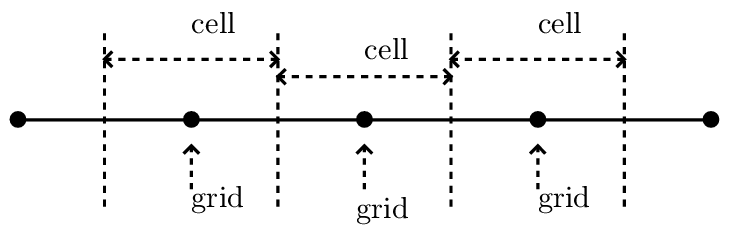
\includegraphics{/home/yj/theory/figures/grids_cells/grids-1.eps}
  \caption{\label{18-11-2-1}Definition of spatial grid points and cells in PIC
  simulations. A grid point is the center of the corresponding cell.}
\end{figure}

Field solvers in PIC code need the values of $I$ at the grid-points. This
value at the grid point is defined as the average of $I$ over the
corresponding cells (similar to that in the finite element method), i.e.,
\begin{equation}
  I_{i, j, k} \equiv I (\alpha_i, \beta_j, \gamma_k) \equiv \frac{1}{\Delta V}
  \int_{\alpha_{i - 1 / 2}}^{\alpha_{i + 1 / 2}} \int_{\beta_{j - 1 /
  2}}^{\beta_{j + 1 / 2}} \int_{\gamma_{k - 1 / 2}}^{\gamma_{k + 1 / 2}} I
  (\alpha, \beta, \gamma) \mathcal{J} d \alpha d \beta d \gamma,
\end{equation}
where $\Delta V = \int_{\alpha_{i - 1 / 2}}^{\alpha_{i + 1 / 2}}
\int_{\beta_{j - 1 / 2}}^{\beta_{j + 1 / 2}} \int_{\gamma_{k - 1 /
2}}^{\gamma_{k + 1 / 2}} \mathcal{J} d \alpha d \beta d \gamma$ is the cell
volume, which can be approximated as $\Delta V \approx \mathcal{J}_{i, j, k}
\Delta \alpha \Delta \beta \Delta \gamma$. Using Eqs. (\ref{3-23-p10}), the
above expression is written as
\begin{equation}
  I_{i, j, k} = \frac{1}{\Delta V} \int_{\alpha_{i - 1 / 2}}^{\alpha_{i + 1 /
  2}} \int_{\beta_{j - 1 / 2}}^{\beta_{j + 1 / 2}} \int_{\gamma_{j - 1 /
  2}}^{\gamma_{j + 1 / 2}} \sum_p w_p A (\mathbf{v}_p) S
  (\mathbf{r}-\mathbf{r}_p) \mathcal{J} d \alpha d \beta d \gamma .
\end{equation}
Using the shape function given in expression (\ref{18-12-19-p1}), the above
expression is written as
\begin{equation}
  \label{18-12-19-p4} I_{i, j, k} = \frac{1}{\Delta V} \sum_p w_p A
  (\mathbf{v}_p) \int_{\alpha_{i - 1 / 2}}^{\alpha_{i + 1 / 2}} \int_{\beta_{j
  - 1 / 2}}^{\beta_{j + 1 / 2}} \int_{\gamma_{j - 1 / 2}}^{\gamma_{j + 1 / 2}}
  \left[ \frac{1}{\Delta \alpha_p} S_{1 D} \left( \frac{\alpha -
  \alpha_p}{\Delta \alpha_p} \right) \right] \left[ \frac{1}{\Delta \beta_p}
  S_{1 D} \left( \frac{\beta - \beta_p}{\Delta \beta_p} \right) \right] \left[
  \frac{1}{\Delta \gamma_p} S_{1 D} \left( \frac{\gamma - \gamma_p}{\Delta
  \gamma_p} \right) \right] d \alpha d \beta d \gamma,
\end{equation}
where the Jacobian in the integrand is cancelled out. The 3D integral in
expression (\ref{18-12-19-p4}) consists of three identical 1D integrations.
Consider one of them:


\begin{equation}
  W = \frac{1}{\Delta \alpha_p} \int_{\alpha_{i - 1 / 2}}^{\alpha_{i + 1 / 2}}
  S_{1 D} \left( \frac{\alpha - \alpha_p}{\Delta \alpha_p} \right) d \alpha,
\end{equation}
Consider the case $\Delta \alpha_p = \Delta \alpha$, and choose $S_{1 D}$ to
be the $l \tmop{th}$ order b-spline function, $b_l$, then the above expression
is written as
\begin{eqnarray}
  W & = & \frac{1}{\Delta \alpha} \int_{\alpha_{i - 1 / 2}}^{\alpha_{i + 1 /
  2}} b_l \left( \frac{\alpha - \alpha_p}{\Delta \alpha} \right) d \alpha 
  \label{18-12-19-e3}\\
  & = & b_{l + 1} \left( \frac{\alpha_i - \alpha_p}{\Delta \alpha} \right), 
  \label{18-12-19-e1}
\end{eqnarray}
where $b_{l + 1}$ is the $(l + 1) \tmop{th}$ order b-spline function. [Proof
of Eq. (\ref{18-12-19-e1}): Using the property of the zeroth order b-spline
function $b_0$ (a flat top function), the integration (\ref{18-12-19-e3}) can
be written as
\begin{eqnarray*}
  W & = & \frac{1}{\Delta \alpha} \int_{- \infty}^{\infty} b_l \left(
  \frac{\alpha - \alpha_p}{\Delta \alpha} \right) b_0 \left( \frac{\alpha -
  \alpha_i}{\Delta \alpha} \right) d \alpha
\end{eqnarray*}
By using the definition of the b-splines, we find the above expression is a
b-spline function that is one order higher than the corresponding b-spline
shape function, i.e.,
\[ W = b_{l + 1} \left( \frac{\alpha_i - \alpha_p}{\Delta \alpha} \right) . \]
] Therefore expression (\ref{18-12-19-p4}) is written as
\begin{equation}
  \label{18-12-19-e10} I_{i, j, k} = \frac{1}{\Delta V} \sum_p w_p A
  (\mathbf{v}_p) b_{l + 1} \left( \frac{\alpha_i - \alpha_p}{\Delta \alpha}
  \right) b_{l + 1} \left( \frac{\beta_j - \beta_p}{\Delta \beta} \right) b_{l
  + 1} \left( \frac{\gamma_k - \gamma_p}{\Delta \gamma} \right) .
\end{equation}
Recall that, in terms of the b-spline functions, the local value $I (\alpha,
\beta, \gamma)$ is given by expression (\ref{3-23-p10}), i.e.,
\begin{equation}
  \label{17-6-26-1} I (\alpha, \beta, \gamma) = \frac{1}{\Delta V} \sum_p w_p
  A (\mathbf{v}_p) b_l \left( \frac{\alpha - \alpha_p}{\Delta \alpha} \right)
  b_l \left( \frac{\beta - \beta_p}{\Delta \beta} \right) b_l \left(
  \frac{\gamma - \gamma_p}{\Delta \gamma} \right) .
\end{equation}
It is instructive to compare expression (\ref{18-12-19-e10}) with
(\ref{17-6-26-1}), which indicates that they are similar except that the
b-spline functions involved in the cell-averaged expression
(\ref{18-12-19-e10}) is one order higher than that involved in the local
expression (\ref{17-6-26-1}).

\subsection{Effective field on a marker}

The effective field on a marker is defined as the averaged field on the group
of particles represented by the marker. To get the averaged field, we need to
reconstruct a continuum electric field from the field values on the discrete
grids.

\subsubsection{Piecewise constant function}

One of many methods of reconstructing the continuum electric field is to
assume that the field is constant in each cell, i.e., piecewise constant
function, i.e.,
\begin{equation}
  \label{2-23-p20} E (\alpha, \beta, \gamma) = \sum_{i, j, k} E_{i, j, k} b_0
  \left( \frac{\alpha - \alpha_i}{\Delta \alpha} \right) b_0 \left(
  \frac{\beta - \beta_i}{\Delta \beta} \right) b_0 \left( \frac{\gamma -
  \gamma_i}{\Delta \gamma} \right),
\end{equation}
where $E_{i, j, k}$ is the field value at grid-points (centers of cells)
obtained by solving the field equation. The electric field on a computational
marker is the average of the electric field over all the physical particles
contained in the marker, i.e.,
\begin{equation}
  E_p = \frac{1}{w_p} \int_{- \infty}^{+ \infty} \int_{- \infty}^{+ \infty}
  \int_{- \infty}^{+ \infty} E (\alpha, \beta, \gamma) \left( \int f_p
  d\mathbf{v} \right) \mathcal{J}_r d \alpha d \beta d \gamma
\end{equation}
Using $f_p$ given in Eq. (\ref{3-23-p12}) in the above equation, we obtain
\begin{equation}
  E_p = \int_{- \infty}^{+ \infty} \int_{- \infty}^{+ \infty} \int_{-
  \infty}^{+ \infty} E (\alpha, \beta, \gamma) \left[ \frac{1}{\Delta
  \alpha_p} S_{1 D} \left( \frac{\alpha - \alpha_p}{\Delta \alpha_p} \right)
  \right] \left[ \frac{1}{\Delta \beta_p} S_{1 D} \left( \frac{\beta -
  \beta_p}{\Delta \beta_p} \right) \right] \left[ \frac{1}{\Delta \gamma_p}
  S_{1 D} \left( \frac{\gamma - \gamma_p}{\Delta \gamma_p} \right) \right] d
  \alpha d \beta d \gamma,
\end{equation}
where the Jacobian and $w_p$ disappear. Use the reconstructed electric field
[Eq. (\ref{2-23-p20})] in the above equation, giving
\begin{equation}
  E_p = \sum_{i, j, k} E_{i, j, k} \int_{- \infty}^{+ \infty} \int_{-
  \infty}^{+ \infty} \int_{- \infty}^{+ \infty} b_0 \left( \frac{\alpha -
  \alpha_i}{\Delta \alpha} \right) b_0 \left( \frac{\beta - \beta_i}{\Delta
  \beta} \right) b_0 \left( \frac{\gamma - \gamma_i}{\Delta \gamma} \right)
  \frac{1}{\Delta \alpha_p} S_{1 D} \left( \frac{\alpha - \alpha_p}{\Delta
  \alpha_p} \right) \frac{1}{\Delta \beta_p} S_{1 D} \left( \frac{\beta -
  \beta_p}{\Delta \beta_p} \right) \frac{1}{\Delta \gamma_p} S_{1 D} \left(
  \frac{\gamma - \gamma_p}{\Delta \gamma_p} \right) d \alpha d \beta d \gamma
\end{equation}
If we choose the shape function $S_{1 D}$ as the b-spline function $b_l$ with
$\Delta \alpha_p = \Delta \alpha$, $\Delta \beta_p = \Delta \beta$, and
$\Delta \gamma_p = \Delta \gamma$, then the above equation is written as
\begin{equation}
  \label{18-12-20-1} E_p = \sum_{i, j, k} E_{i, j, k} b_{l + 1} \left(
  \frac{\alpha_i - \alpha_p}{\Delta \alpha} \right) b_{l + 1} \left(
  \frac{\beta_j - \beta_p}{\Delta \beta} \right) b_{l + 1} \left(
  \frac{\gamma_k - \gamma_p}{\Delta \gamma} \right),
\end{equation}
which specifies how the effective field on a marker is related to the nearby
field on the grid-points.

\subsubsection{Piecewise linear function}

Another way of reconstructing the continuum electric field is to assume that
the field is linear function between grids. In this case, if the spatial shape
function of markers is Dirac delta function, then it is obvious that the
effective field on a marker can be obtained by linearly interpolating the
fields on the nearyby grids. If the spatial shape function of markers is
$b_0$, what is the interpolation scheme of obtaining the effective field on a
marker? To be worked out. The result will be a little complicated than the
linear interpolation and thus involves more computational overhead. The
benefit can be that the noise can be further reduced, compared with the linear
interpolation.

\subsection{Effective force on a marker}

The total charge of a group of particles represented by a maker, $Q$, is given
by $Q = \int q f_p d^6 v$, where $q$ is the charge of a single particle. Then
the effective force on a marker is then $F_p = Q E_p$ with $E_p$ given by Eq.
(\ref{3-24-a1}). The total mass of a group of particles represented by a
marker, $M$, is given by $M = \int m f_p d^6 v$, where $m$ is the mass of a
single particle. Then the ratio between $Q$ and $M$ is written as
\begin{equation}
  \frac{Q}{M} = \frac{\int q f_p d^6 v}{\int m f_p d^6 v} = \frac{q}{m},
\end{equation}
which is identical to the single particle charge mass ratio. Note that the
motion equation of a particle in an electromagnetic field is distinguished
only by this ratio. Therefore motion of a marker in the phase space is
identical with the motion of a real particle with the effective field given by
Eq. (\ref{3-24-a1}).

\subsection{Numerical implementation in codes}

Most PIC codes use the $l = 0$ b-spline function (i.e., $b_0$, the flat-top
function) as the shape function of markers. This model is often called Could
in Cell (CIC) since a particle looks like a finite-sized cloud rather than a
point. In this case, the cell average of $I$ given in Eq. (\ref{18-12-19-e10})
is written as
\begin{equation}
  \label{3-24-a3} I_{i, j, k} = \frac{1}{\Delta V} \sum_p w_p A (\mathbf{v}_p)
  b_1 \left( \frac{\alpha_i - \alpha_p}{\Delta \alpha} \right) b_1 \left(
  \frac{\beta_j - \beta_p}{\Delta \beta} \right) b_1 \left( \frac{\gamma_k -
  \gamma_p}{\Delta \gamma} \right)
\end{equation}
and the electric field on the marker given in Eq. (\ref{18-12-20-1}) is
written as
\begin{equation}
  \label{3-24-a4} E_p = \sum_{i, j, k} E_{i, j, k} b_1 \left( \frac{\alpha_i -
  \alpha_p}{\Delta \alpha} \right) b_1 \left( \frac{\beta_j - \beta_p}{\Delta
  \beta} \right) b_1 \left( \frac{\gamma_k - \gamma_p}{\Delta \gamma} \right),
\end{equation}
Because the function $b_1$ has a narrow support, as shown in Fig.
\ref{17-6-25-p1}, in practice of calculating $I_{i, j, k}$ in expression
(\ref{3-24-a3}), we loop over each particle for only once and assign the
contribution of each one to their neighbouring cells (rather than looping over
all particle for each cell as the straightforward reading of expression
(\ref{3-24-a3}) would suggest). The operation of the latter would be $O (N
\times N_p)$, where $N$ is number of grids and $N_p$ is the number of markers,
while the former is only $O (n N_p)$, where $n$ is the number of operation
involved in assigning each particle to its neighbouring cells, which is
usually much smaller than the grid number $N$.

Similarly, in calculating the force on a marker, the summation over all the
grids (as the straightforward reading of expression (\ref{3-24-a4}) would
suggest) is not needed. We only need to find which cell a marker is in and
then sum the contribution from the nearby grids (rather than all the grids).

\subsection{Monte-Carlo integration in phase-space}

Consider a general integration of the distribution function $f$ in the
phase-space
\begin{equation}
  \label{16-3-22-p2} I \equiv \int_{\Omega'} A (\mathbf{Z}) f (\mathbf{Z}) d
  V,
\end{equation}
where $\Omega'$ is a sub-region of the phase space $\Omega$, $A (\mathbf{Z})$
is a general function of the phase-space coordinates $\mathbf{Z}$, $d V$ is
the phase space volume element. As is discussed above, in particle methods, $f
(\mathbf{Z})$ is approximated by
\begin{equation}
  f (\mathbf{Z}) \approx \sum_{j = 1}^N w_j S_{\tmop{ps}}
  (\mathbf{Z}-\mathbf{Z}_j),
\end{equation}
where $S_{\tmop{ps}} (\mathbf{Z}-\mathbf{Z}_j)$ is the phase space shape
function of markers, $N$ is the total number of marker loaded in the phase
space $\Omega$. Using this, expression (\ref{16-3-22-p2}) is written as
\begin{equation}
  \label{17-7-17-p5} I = \sum_{j = 1}^N \int_{\Omega'} A (\mathbf{Z}) w_j
  S_{\tmop{ps}} (\mathbf{Z}-\mathbf{Z}_j) d V,
\end{equation}
If the shape function $S_{\tmop{ps}}$ is chosen to be the Dirac delta
function, then the above equation is written as


\begin{equation}
  \label{17-6-13-3} I = \sum_{j = 1}^{N'} A (\mathbf{Z}_j) w_j,
\end{equation}
where $N'$ is the number of markers that are within the sub-region $\Omega'$.
Equation (\ref{17-6-13-3}) is the Monte-Carlo approximation to the integration
in Eq. (\ref{16-3-22-p2}){\cite{Fitzpatrickcp,aydemir1994}}.

In PIC simulations, we are usually interested in velocity moments of $f$
averaged in a cell, i.e., $\mathbf{A}$ in Eq. (\ref{17-7-17-p5}) is only a
function of only $\mathbf{v}$ and the velocity integration is over the whole
velocity space, whereas the spatial integration is over a small spatial cell.
Furthermore, in PIC simulations, the markers are assumed to have a finite
shape in the real space (the shape in velocity space is still the Dirac delta
function). In this case, Eq. (\ref{17-7-17-p5}) is written as
\begin{eqnarray}
  I & = & \sum_{j = 1}^N \int_{\mathbf{v}} A (\mathbf{v}) w_j \delta
  (\mathbf{v}-\mathbf{v}_j) \left( \int_{\Delta V_r} S_r
  (\mathbf{r}-\mathbf{r}_j) d\mathbf{r} \right) d\mathbf{v}, \nonumber\\
  & = & \sum_{j = 1}^N A (\mathbf{v}_j) w_j  \left( \int_{\Delta V_r} S_r
  (\mathbf{r}-\mathbf{r}_j) d\mathbf{r} \right), 
\end{eqnarray}
where $S_r$ is the shape function. Then the cell-averaged value is written as
\begin{equation}
  \frac{I}{\Delta V_r} = \sum_{j = 1}^N A (\mathbf{v}_j) w_j  \left(
  \frac{1}{\Delta V_r} \int_{\Delta V_r} S_r (\mathbf{r}-\mathbf{r}_j)
  d\mathbf{r} \right) .
\end{equation}


\subsection{On accuracy and noise: particle methods vs. Euler-grid-based
methods}

The overall error of the Monte-Carlo approximation given in Eq.
(\ref{17-6-13-3}) always scales like $1 / \sqrt{N'}$, which is independent of
the dimensionality of the phase-space. It is easy to demonstrate that the
overall error of the usual regular-grids approximation to the integration
scales like $1 / N^{\prime 1 / d}$, where $d$ is the dimension of the phase
space{\cite{Fitzpatrickcp}}. This fact implies that Monte-Carlo approximation
is more accurate than the regular-grids methods for high-dimension $(d
\geqslant 3)$ integration. Due to this reason, particle methods can be
considered more accurate than the Euler-grid-based methods for the same number
of sampling points in a high-dimensional $(\geqslant 3)$ phase space.

On the other hand, PIC simulations obviously contain unphysical noise. The
noise is due to the discrete marker effects, which can be further categorized
into two types: sampling noise (fluctuation of the sampling error) and
remaining unwanted collisions in a collisionless simulation.

Due to the limited small number of markers used in PIC code, there are
considerable time and spatial fluctuation over the the number of markers in a
spatial-cell. This fluctuation in the number of sampling points (i.e.,
fluctuation of the sampling error) gives rise to the sampling noise.

Inaccuracy in a PIC simulation is also related to the fact that the
phase-space volume sampled by a marker is assumed to be constant in a PIC code
but this assumption is not strictly satisfied in practice due to (1) the
number of markers being not large enough and (2) the resulting self-consistent
field being not smooth enough, which introduce effective collisional effects,
making the conservation of the phase-space volume less accurate. How well the
phase-space volume is conserved depends on the smoothness of the field: smooth
field means less collisions and thus phase-space volume are better conserved.
PIC simulation codes seek to reduce the collision through using finite-size
particles (discussed in Sec. \ref{16-3-29-a5}) and averaging in a spatial cell
in solving for the electromagnetic fields, which effectively smooth the
fields. This kind of PIC simulations are thus designed for collisionless
plasmas. And the remaining collisional effect should be small enough to not
affect the process of interest. And this remaining collisional effects should
be viewed as numerical artifacts rather than a modeling of any real
collisional effect in plasmas. If we want to model the real collisional effect
in PIC simulation, we need to use other techniques rather than relying on the
remaining collisions mentioned above because the latter is not easy to control
and ideally should be completely removed.

Various noise reduction techniques in PIC codes (e.g., finite-size particles,
grids, and perturbative $\delta f$ method) can be used when the marker number
is fixed. When exhausting all these methods, the final brute-force method of
reducing noise (reducing collisions) is to increase the marker number.
Therefore the noise issue is finally a convergence issue about the marker
number.

From the view of particle simulations, the gyrokinetic model can also be
considered as a noise reduction technique, where the gyro-averaging process
makes the field on a marker more smooth.

(Noise in PIC code is equivalent to the remaining artificial collision effect?
We can test this by doing a test particle simulation, in which we loaded a
group of markers to sample a distribution function in the phase space and then
compute the density evolution of the sampled distribution under a given smooth
electromagnetic field (i.e., eliminating the collisional effect). If there is
still significant noise in the time evolution, then this indicates there are
factors other than collisions that contribute to the noise. I did this when I
studied Landau damping, the results indicate there is still significant noise
in the solution, indicating the discrete phase space sampling is the root of
the noise.)

One thing to note is that the noisy results obtained in particle method are
not necessarily less accurate than the smooth results obtained in
Euler-grid-based methods because bigger errors may be hidden in smooth results
when one uses coarse grids.

\subsection{Practical comparison between particle methods and Euler-grid-based
methods}

Kinetic plasma simulations in a 6D phase space is usually difficult for
grid-based methods because the six-dimensional phase space seems to be too
high for Euler-gird-based methods to handle. As a result, I have not seen any
6D grid-based kinetic simulation code. With the invention of the gyrokinetic
model, the dimenionality of the phase space is reduced to five, which makes it
possible for Euler-grid-based method to handle. As a result, there appear
several widely used gird-based gyrokinetic codes, such as \tmtexttt{GYRO} and
\tmtexttt{GENE}.

Another reason why particle methods are (if they are) more popular than the
Eulerian-grid-based methods in plasma community is the algorithmic compactness
and subsequent ease of coding in comparison with the Eulerian-grid-based
methods. The popularity of PIC methods may also be related to that PIC method
seems more intuitive at first glance (although this first impression may be
only partially correct and even misleading). This is not about accuracy or
even science. Historical or psychological reasons can partially account for
the popularity of one particular method.

Parallization of the marker pushing part is usually easy in PIC codes. All the
markers used in a simulation can be evenly distributed among all the MPI
processes used. The loading balance can be good among all the processes in
terms of marker pushing. The deposition part of a PIC code can be slow because
it involves random access to a large grid array when looping over all the
markers in a MPI process. The parallization of the field solving part is the
same as Euler based codes.

For gyrokinetic simulation of tokamak plasmas, it is not easy to judge which
method, particle-based method or grid-based mthod, is better than the other.
When dealing with full Landau collision oprators, some PIC codes, e.g.,
\tmtexttt{XGC}, uses velocity space grids. This may indicate that velocity
grids are generally needed, suggesting that grids-methods may have advantages.
On the other hand, hybrid methods that use both velocity grids and markers may
be a practical way since ``hybrid'' provides us freedoms to use whatever
methods available that can get work done.

\subsection{Modeling collisions in PIC simulations}

(check**However, the grid-less approach in particle method makes it difficult
to handle general Landau collision operators that involve the velocity
gradients of the distribution function and evaluating these gradients usually
needs velocity grids. For some simple collision operators, a corresponding
Langevin equation can be constructed, which makes the collisional effect be
able to be modeled by stochastic change in marker trajectories. However, this
correspondence can not be found for all collisional operators.)

\section{Evolution of distribution functions}

The marker weight is composed of two factors, namely the physical distribution
function $f$ and the marker distribution function $g$. The time evolution of
the weight $w$ is thus determined by the time evolution of $f$ and $g$, which
are discussed in Sec. \ref{16-5-26-1} and \ref{16-5-26-2}, respectively.)

\subsection{Time evolution of the physical distribution
function}\label{16-5-26-1}

\subsubsection{Full-f formula}

The collisionless kinetic equation (Vlasov equation) is given by
\begin{equation}
  \label{17-3-13-e1} \frac{\partial f}{\partial t} +\mathbf{v} \cdot
  \frac{\partial f}{\partial \mathbf{x}} + \frac{q}{m} (\mathbf{E}+\mathbf{v}
  \times \mathbf{B}) \cdot \frac{\partial f}{\partial \mathbf{v}} = 0,
\end{equation}
It is ready to find that the characteristic lines of the equation is given by
\begin{equation}
  \label{17-3-13-e2} \frac{d\mathbf{x}}{d t} =\mathbf{v},
\end{equation}
and
\begin{equation}
  \label{17-3-13-e3} \frac{d\mathbf{v}}{d t} = \frac{q}{m}
  (\mathbf{E}+\mathbf{v} \times \mathbf{B}) .
\end{equation}
Along a characteristic line, the kinetic equation is written
\begin{equation}
  \label{3-8-p1} \frac{d f}{d t} = 0,
\end{equation}
where $f$ is the total particle distribution function (full-f). Particles
methods that use Monte-Carlo sampling to approximate the total $f$ are called
total-f or full-f method.

\subsubsection{Delta-f formula}

Since the phenomena we consider in tokamak plasmas are usually developing from
an equilibrium or near-equilibrium state, it is desirable to calculate the the
evolution of the only the perturbation, instead of the total $f$. Therefore,
we write $f$ as the sum of a known time-independent distribution function
$f_0$ ($\partial f_0 / \partial t$=0) and a unknown time-dependent
perturbation $\delta f$ $(\partial \delta f / \partial t \neq 0)$:
\begin{equation}
  \label{10-26-e1} f = f_0 + \delta f,
\end{equation}
Then the kinetic equation (\ref{3-8-p1}) is written
\begin{equation}
  \label{3-8-p3} \frac{d \delta f}{d t} = - \frac{d f_0}{d t} .
\end{equation}
Particle methods that use Monte-Carlo sampling to approximate the \ $\delta f$
are usually called $\delta f$ method. When the right-hand side of Eq.
(\ref{3-8-p3}) is known, Eq. (\ref{3-8-p3}) can be integrated to obtain the
time evolution of $\delta f$. The time evolution of $\delta f$ can also be
obtained by using
\begin{equation}
  \label{17-6-12-p9} \delta f (t, \mathbf{Z}_j (t)) = f (t = 0, \mathbf{Z}_j
  (t = 0)) - f_0 (\mathbf{Z}_j (t)) .
\end{equation}
In this way, the time integration of $\delta f / d t$ is avoided, which may
reduce the computational overhead and improve the accuracy of $\delta f$. This
seemingly trivial method was emphasized in a CPC paper{\cite{allfrey2003}},
which introduces an adaptive $f_0$ method based on this idea. I have tested
this method in my toy code about the 1D Landau damping, which gave the same
results as the usual method. However, Yang Chen pointed out that this method
is never used in simulations of tokamak plasmas due to the following reasons.
The chosen equilibrium distribution function $f_0$ in tokamak plasmas
simulation is usually not a solution the following time-independent Vlasov
equation:
\begin{equation}
  \mathbf{v} \cdot \frac{\partial f_0}{\partial \mathbf{x}} + \frac{q}{m}
  (\mathbf{E}_0 +\mathbf{v} \times \mathbf{B}_0) \cdot \frac{\partial
  f_0}{\partial \mathbf{v}} = 0,
\end{equation}
Instead, the chosen $f_0$ is a solution of the following equation
\begin{equation}
  \label{17-6-12-p4} \mathbf{v} \cdot \frac{\partial f_0}{\partial \mathbf{x}}
  + \frac{q}{m} (\mathbf{E}_0 +\mathbf{v} \times \mathbf{B}_0) \cdot
  \frac{\partial f_0}{\partial \mathbf{v}} = S,
\end{equation}
where $S$ is a nonzero term. On the other hand, the perturbation part is
governed by the following equation
\begin{equation}
  \frac{d \delta f}{d t} = - \frac{q}{m} (\delta \mathbf{E}+\mathbf{v} \times
  \delta \mathbf{B}) \cdot \frac{\partial f_0}{\partial \mathbf{v}} .
\end{equation}
Then it is ready to prove that the actual kinetic equation for the full $f$ in
the usual tokamak simulation is actually given by
\begin{equation}
  \label{17-6-12-p11} \frac{d f}{d t} = S,
\end{equation}
which indicates that $f$ is not a constant along the characteristic curves and
thus is not consistent with the algorithm given in Eq. (\ref{17-6-12-p9}).
**may be wrong, check**The case given in Eq. (\ref{17-6-12-p11}) is the more
relevant case to tokamak experiments where a particular form of $f_0$ is
maintained by external sources and we are asked to calculate the perturbation
evolution around $f_0$.**wrong!

\subsection{Time evolution of marker distribution function}\label{16-5-26-2}

For Hamiltonian motion in particular and non-diffusive motion in general, any
particle distribution function $g (\mathbf{x}, \mathbf{v}, t)$ satisfies that
$d g / d t = 0$. In other words, the phase-space particle flow is volume
preserving (this is Louisville's theorem), i.e.,
\begin{equation}
  \label{16-5-26-3} \frac{d V_j}{d t} = 0.
\end{equation}
i.e, the phase-space volume sampled by a marker does not change along the
characteristic curves. This is good news for PIC simulation because this means
that the marker distribution is known exactly along the characteristic line at
every time-step and we do not need to numerically evaluate it (numerically
evaluating the marker distribution by directly counting markers would be noisy
due to the small number of markers loaded and should be avoided in practice
whenever possible).

For diffusive motion, the phase space particle flow is usually not volume
preserving, i.e.,
\begin{equation}
  \frac{d g (\mathbf{Z}_j)}{d t} \neq 0.
\end{equation}
For this case, the values of $g$ at markers need to be evaluated numerically
every time step, which is usually noisy and time-consuming in terms of CPU
time. Therefore, this kind of evaluation should be avoided in practice
whenever possible. The usual way of achieving this is by choosing a suitable
initial distribution for the markers, so that $g$ remains approximately
constant along the trajectory of markers{\cite{chen1997}}.

The marker distribution chosen in practice is determined by the desired
resolution of phase space of interest, not determined by the physical particle
distribution, i.e., the initial marker distribution can be different from the
physical particle distribution.

\subsection{Time evolution of marker's weight}

As mentioned in Sec. \ref{16-8-19-p1}, marker's weight, $w = f / g$, is
composed of two factors, namely the physical distribution function $f$ and the
markers' distribution function $g$. The time evolution of the weight $w$ is
thus determined by the time evolution of $f$ and $g$.. In some cases, the
formula for the time evolution of both $f$ and $g$ can be obtained
analytically, as discussed in Sec. \ref{16-5-26-1} and \ref{16-5-26-2},
respectively. [*check**In other cases, the formula for the time evolution of
$f$ and/or $g$ can not be easily obtained but the formula for the time
evolution of $w$ can still be obtained analytically. A typical example of this
kind is the full-f simulation including the collision effects in the orbits.
In this case, the phase-space flow is not volume-conserving, i.e., $d g / d t
\neq 0$, and it is difficult to find an analytic formula for the time
evolution of $g$. However, the conservation of the particle number along the
orbits in the phase space is still valid (check this!, wrong), i.e.,
\begin{equation}
  \frac{d w}{d t} = 0.
\end{equation}


Does this algorithm correctly describe the ``collision''? This algorithm
(i.e., including the collision effects via randomly changing the orbit
variables) is obviously correct when $w$ is 1, i.e., a marker only represents
one physical particle. The correctness for $w_j > 1$ case should be verified.
***check]. Collisions in both full-f and $\delta f$ methods seem to be
implemented by including a source term in the evolution equation for the
weight, rather than kicking the orbit (I will check the kicking orbit method
later).

\section{An example: One-dimensional electrostatic simulation}

\subsection{Vlasov equation}

Consider the electrostatic case. The Vlasov equation (\ref{10-13-1a}) for
electrons is written
\begin{equation}
  \frac{\partial f}{\partial t} +\mathbf{v} \cdot \nabla f + \frac{e}{m}
  \nabla \phi \cdot \nabla_v f = 0,
\end{equation}
where $\phi$ is the electric potential. Consider the one-dimensional case
where $f$ and $\phi$ are independent of $y$ and $z$ coordinates. In this case,
the above equation is written
\begin{equation}
  \frac{\partial f}{\partial t} + v_x \frac{\partial f}{\partial x} +
  \frac{e}{m}  \frac{d \phi}{d x}  \frac{\partial f}{\partial v_x} = 0
\end{equation}
Integrating both sides of the above equation over $v_y$ and $v_z$, we obtain
\begin{equation}
  \label{10-7-e1} \frac{\partial F}{\partial t} + v_x \frac{\partial
  F}{\partial x} + \frac{e}{m}  \frac{d \phi}{d x}  \frac{\partial F}{\partial
  v_x} = 0,
\end{equation}
where $F (x, v_x, t) = \int_{- \infty}^{\infty} \int_{- \infty}^{\infty} f d
v_y d v_z$ is the reduced distribution function. Define characteristic lines
by the following ordinary differential equations:
\begin{equation}
  \label{10-10-1} \frac{d x}{d t} = v_x,
\end{equation}
and
\begin{equation}
  \label{10-10-2} \frac{d v_x}{d t} = \frac{e}{m_e}  \frac{d \phi}{d x} .
\end{equation}
Then along a characteristic line, we obtain
\begin{equation}
  \label{10-10-3} \frac{d F}{d t} = 0,
\end{equation}
which indicates that the distribution function $F$ remain unchanged along a
characteristic line.

\subsection{Poisson's equation}

In terms of the reduced distribution function $F$, Poisson's equation is
written
\begin{equation}
  \label{10-10-4} - \frac{d^2 \phi}{d x^2} = \frac{e}{\varepsilon_0} \left(
  n_{\tmop{ion}} - \int_{- \infty}^{\infty} F d v_x \right),
\end{equation}
where $n_{\tmop{ion}}$ is the number density of ions, which are assumed to be
uniform in $x$ and not evolving with time.

\subsection{Equilibrium state}

Consider a spatially uniform distribution function given by
\begin{equation}
  \label{16-3-29-a1} F (x, v_x, t) = F_0 (v_x),
\end{equation}
where $F_0 (v_x)$ is a known velocity distribution function with number
density being equal to those of ions, i.e., $\int_{- \infty}^{+ \infty} F_0
(v_x) d v_x = n_{\tmop{ion}}$. Consider a case with zero electric field, i.e.,
\begin{equation}
  \label{16-3-29-a2} E (x, t) = 0.
\end{equation}
Then it is ready to verify that expression specified by Eqs.
(\ref{16-3-29-a1}) and (\ref{16-3-29-a2}) is a equilibrium solution to
Vlasov-Poisson system (Eqs. (\ref{10-7-e1}) and (\ref{10-10-4})).

In this note, two kind of equilibrium distribution functions will be
considered. The first one is the Maxwellian distribution given by
\begin{equation}
  F_0 (v_x) = \frac{n_{e 0}}{\sqrt{\pi} v_t} \exp \left( - \frac{v^2}{v_t^2}
  \right) .
\end{equation}
In this system, small perturbation will be damped by a mechanism known as
Landau damping. The second kind of distribution considered is the two-stream
Maxwellian distribution given by
\begin{equation}
  F_0 (v_x) = \frac{n_{e 0}}{\sqrt{\pi} v_t}  \frac{1}{2} \left[ \exp \left( -
  \frac{(v - v_b)^2}{v_t^2} \right) + \exp \left( - \frac{(v + v_b)^2}{v_t^2}
  \right) \right] .
\end{equation}
In this system, small perturbation will give rise to an instability known as
the two-stream instability.

\subsection{$\delta f$ evolution}

Write the distribution function $F$ as
\begin{equation}
  F = F_0 + \delta F,
\end{equation}
where $F_0$ is the equilibrium distribution function. Then Eq. (\ref{10-10-3})
is written as
\begin{equation}
  \label{16-4-21-1} \frac{d \delta F}{d t} = - \frac{d F_0}{d t} .
\end{equation}
Use the definition of the orbit propagator,
\begin{equation}
  \frac{d}{d t} \equiv \frac{\partial}{\partial t} + v_x
  \frac{\partial}{\partial x} + \frac{e}{m}  \frac{d \phi}{d x} 
  \frac{\partial}{\partial v_x},
\end{equation}
to rewrite the right-hand side of Eq. (\ref{16-4-21-1}), yielding
\begin{equation}
  \label{3-25-a5} \frac{d \delta F}{d t} = - \left( \frac{e}{m}  \frac{d
  \phi}{d x}  \frac{\partial F_0}{\partial v_x} \right),
\end{equation}
which can be integrated to obtain the time evolution of $\delta F$.

The time evolution of $\delta F$ can also be obtained by using
\begin{equation}
  \label{17-7-21-1} \delta F (\mathbf{Z}_j (t)) = F (\mathbf{Z}_j (t = 0)) -
  F_0 (\mathbf{Z}_j (t)) .
\end{equation}
In this way, the time integration of $\delta F / d t$ is avoided, which may
reduce the computational work load and improve the accuracy of $\delta F$.
This seemingly trivial method was emphasized in a CPC
paper{\cite{allfrey2003}}, which introduces an adaptive $F_0$ method based on
this idea. I have compared the results of Landau damping obtained by the two
methods (i.e., using Eq. (\ref{3-25-a5}) and Eq. (\ref{17-7-21-1}),
respectively), which shows they agree with each other very well.

\subsection{Normalization}\label{3-25-a4}

Choose a typical number density $n_0$ and a typical velocity $v_0$, then
define the electron plasma frequency $\omega_{p e}$ and the Debye length
$\lambda_D$ as
\begin{equation}
  \omega_{p e} = \sqrt{\frac{n_0 e^2}{m_e \varepsilon_0}},
\end{equation}
and
\begin{equation}
  \lambda_D = \frac{v_0}{\omega_{p e}},
\end{equation}
respectively. Using $\omega_{p e}$ and $\lambda_D$, define the following
normalized quantities:
\begin{equation}
  \overline{t} = t \omega_{p e}, \overline{x} = \frac{x}{\lambda_D},
  \overline{\phi} = \frac{e \phi}{m_e v_0^2}, \overline{F} = \frac{v_0}{n_0}
  F, \overline{v}_x = \frac{v_x}{v_0} \nocomma, \overline{n}_i =
  \frac{n_i}{n_0}
\end{equation}
In terms of these normalized quantities, equation (\ref{10-10-3}) is written
\begin{equation}
  \label{2-12-1} \frac{d \overline{F}}{d \overline{t}} = 0,
\end{equation}
and the Poisson equation (\ref{10-10-4}) is written
\begin{equation}
  \label{11-4-p1} \frac{d^2 \overline{\phi}}{d \overline{x}^2} = -
  \overline{\rho} .
\end{equation}
where $\overline{\rho} = \overline{n}_{\tmop{ion}} - \int_{- \infty}^{\infty}
\overline{F} d \overline{v}_x$.

The equations for the characteristic lines, Eq. (\ref{10-10-1}) and
(\ref{10-10-2}), are written
\begin{equation}
  \label{12-24-1} \frac{d \overline{x}}{d \overline{t}} = \overline{v}_x,
\end{equation}
\begin{equation}
  \label{12-24-2} \frac{d \overline{v}_x}{d \overline{t}} = \frac{d
  \overline{\phi}}{d \overline{x}} .
\end{equation}
The electric field is given by $E = - d \phi / d x$, which, in terms of
normalized quantities, is written
\begin{equation}
  \overline{E} = - \frac{d \overline{\phi}}{d \overline{x}},
\end{equation}
where $\overline{E} = E e \lambda_D / (m v_0^2)$.

In terms of the normalized quantities, the evolution equation (\ref{3-25-a5})
of $\delta F$ is written as
\begin{equation}
  \label{16-3-1-1} \frac{d \delta \overline{F}}{d \overline{t}} = \overline{E}
  \frac{\partial \overline{F}_0}{\partial \overline{v}_x}
\end{equation}
In terms of $\delta \overline{F}$, Poisson's equation is written as
\begin{equation}
  \frac{d \overline{\phi}}{d \overline{x}^2} = \int_{- \infty}^{\infty} \delta
  \overline{F} d \overline{v}_x,
\end{equation}
where $n_{\tmop{ion}} = n_{e 0}$ has been assumed.

\

\subsection{Boundary condition for field}

The periodic boundary condition is used for the electrical field $E$, i.e.,
the electric field on the right boundary is set equal to that on the left
boundary.

\subsection{Boundary condition for particles}

The periodic boundary condition is also used for markers, i.e., a marker that
leaves from the right boundary will re-enter the computational region from the
left boundary and vice versa.

\subsection{Evaluation of particle number density}\label{10-12-e1}

Set up uniform grid-points in $x$-direction: $x_j = j \Delta$ for $j = 0, 1,
2, \ldots, N$, as is shown in Fig. \ref{16-2-25-p3}. Use the first b-spline
(flat-top function) with a support $\Delta_p = \Delta$ as the shape function
of markers. It is obvious that we can use the following procedures to obtain
the number of physical particles in each cell. For a particle marker labeled
by $k$ whose position is $x = r$, we can find which two grids the particle
lies between. Suppose that $r$ is between $x_j$ and $x_{j + 1}$, then the
particle number $n_j$ and $n_{j + 1}$ is evaluated as follows
\begin{equation}
  \label{10-13-1} n_j \rightarrow n_j + w_k \cdot \frac{x_{j + 1} -
  r}{\Delta}, n_{j + 1} \rightarrow n_{j + 1} + w_k \cdot \frac{r -
  x_j}{\Delta},
\end{equation}
where $w_k$ is the weight of the marker. Performing the same procedures for
each marker in turn allows us to build up $n_j$ at all the grid points (all
$n_j$ are set to zero before these procedures).

The particle number at the boundary grid-points $j = 0$ and $j = N$ needs
special treatment. The above treatment do not include the contribution to
$n_0$ from the left cell of the $j = 0$. Since we use periodic boundary
condition, the contribution to $n_0$ from the left cell of the $j = 0$ grid is
identical to the contribution to $n_N$ from the left cell of the $j = N$ grid.
The latter has already been calculated in the above, which can be added to
$n_0$ obtained above to get the final $n_0$. The same situation applies for
$n_N$. After these treatment, we have $n_0 = n_N$.

Dividing the particle number $n_j$ by the cell size $\Delta$ gives the number
density.

\subsection{FFT solver for Poisson equation}

The normalized one-dimensional Poisson equation is given by Eq.
(\ref{11-4-p1}). For notation simplicity, omit the over-bar on $\phi$ and $x$,
then Eq. (\ref{11-4-p1}) is written
\begin{equation}
  \label{10-11-1} \frac{d^2 \phi}{d x^2} = - \rho .
\end{equation}
This is a two-points boundary value problem. Two boundary conditions are
needed to determine the solution. Assume the periodic boundary condition $\phi
(0) = \phi (L)$ and note that $\phi$ can contain an arbitrary constant. Thus
the periodic boundary condition alone is sufficient to specify the electrical
field. We use Fourier transformation method to solve Eq. (\ref{10-11-1}). The
Fourier transformation of the left-hand side of the above equation is written
\begin{eqnarray}
  \int_{- \infty}^{\infty} \frac{d^2 \phi}{d x^2} e^{i k x} d x & = & - k^2
  \int_{- \infty}^{\infty} \phi e^{i k x} d x \nonumber\\
  & = & - k^2 \hat{\phi} (k), 
\end{eqnarray}
where $\hat{\phi}$ is the Fourier transformation of $\phi$. Using this, the
Fourier transformation of Eq. (\ref{10-11-1}) is written
\begin{equation}
  \label{10-11-p5} \hat{\phi} (k) = \frac{\hat{\rho} (k)}{k^2},
\end{equation}
where
\begin{equation}
  \label{10-11-p1} \hat{\rho} = \int_{- \infty}^{\infty} \rho (x) e^{i k x} d
  x
\end{equation}
is the Fourier transformation of $\rho$. After $\hat{\phi}$ is obtained, the
electric potential $\phi$ is finally reconstructed via the inverse Fourier
transformation
\begin{equation}
  \label{10-11-p2} \phi = \frac{1}{2 \pi} \int_{- \infty}^{\infty} \hat{\phi}
  (k) e^{- i k x} d k.
\end{equation}
In the numerical implementation, the Fourier transformation in Eq.
(\ref{10-11-p1}) and the inverse transformation in Eq. (\ref{10-11-p2}) are
discretized by the Discrete Fourier Transformation (DFT), which is further
evaluated by using the FFT algorithm (I use the FFTW library). Set up uniform
grid-points in $x$-direction: $x_j = j \Delta$ for $j = 0, 1, 2, \ldots, N$,
as is shown in Fig. (\ref{16-2-25-p3}).

\begin{figure}[h]
  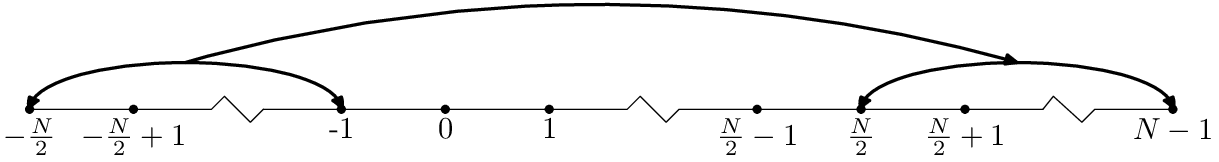
\includegraphics{/home/yj/project_new/fft/fig2d/MyFigure.eps}
  \caption{\label{16-2-25-p3}One-dimensional spatial computational box and
  grids.}
\end{figure}

Let $\rho_j = \rho (x_j)$ and $\phi_j = \phi (x_j)$. Let $\hat{\rho}_j$ and
$\hat{\phi}_j$ denote the corresponding DFT. Using the sampled points $\rho_j$
with $j = 0, 1, 2, \ldots, N - 1$, we can obtain the DFT $\hat{\rho}_j$. Note
that the corresponding wave-number $k$ of $\hat{\rho}_j$ (also for
$\hat{\phi}_j$) is given by $k = j 2 \pi / (N \Delta)$ for $j = 0, 1, \ldots,
N / 2$ and $k = (j - N) 2 \pi / (N \Delta)$ for $j = N / 2 + 1, \ldots, N - 1$
(this corresponds to the negative wave-number part). Use Eq. (\ref{10-11-p5})
and the corresponding expression of the wave-number, the discrete form of Eq.
(\ref{10-11-p5}) is written
\begin{equation}
  \label{16-3-25-a8} \hat{\phi}_j = \frac{\hat{\rho}_j}{[j 2 \pi / (N
  \Delta)]^2} .
\end{equation}
for $j = 1, 2, \ldots, N / 2$, and
\begin{equation}
  \label{16-3-25-a9} \hat{\phi}_j = \frac{\hat{\rho}_j}{[(j - N) 2 \pi / (N
  \Delta)]^2}
\end{equation}
for $j = N / 2 + 1, N / 2 + 2, \ldots, N - 1$. The $j = 0$ case is a special
one because in this case $k = 0$ and $k$ appears in the denominator of
(\ref{10-11-p5}). Since the overall charge neutrality$\int_{- \infty}^{\infty}
\rho d x = 0$ implies $\hat{\rho}_0 = 0$. we usually set $\hat{\phi}_0 = 0$.
After obtaining $\hat{\phi}_j$ with $j = 0, 1, \ldots, N - 1$, we can obtain
$\phi_j$ through the inverse DFT.

Knowing the electron potential $\phi_j$, the electric field is obtained
through the following central difference scheme
\begin{equation}
  \left. E_j = - \frac{d \phi}{d x} \right|_{x = x_j} = - \frac{\phi_{j + 1} -
  \phi_{j - 1}}{2 \Delta} .
\end{equation}
The electric field at the boundary points are obtained by using the periodic
boundary conditions of $\phi$.

In the above we use Fourier transformation method to get the electric
potential and then use finite difference scheme to calculate the electric
field. This is a mixed way to calculate the electric field. We can use only
Fourier transformation method to solve for the electric field. In terms of the
electric field, Poisson equation (\ref{11-4-p1}) is written
\begin{equation}
  \frac{d \overline{E}}{d \overline{x}} = \overline{\rho} .
\end{equation}
For notation simplicity, omit the over-bar on variables, the above equation is
written
\begin{equation}
  \label{2-26-e1} \frac{d E}{d x} = \rho .
\end{equation}
The Fourier transformation of the left-hand side of the above equation is
written
\begin{eqnarray}
  \int_{- \infty}^{\infty} \frac{d E}{d x} e^{i k x} d x & = & \int_{-
  \infty}^{\infty} e^{i k x} d E \nonumber\\
  & = & E e^{i k x} |_{- \infty}^{+ \infty} \nobracket - i k \int_{-
  \infty}^{\infty} E e^{i k x} d x \nonumber\\
  & = & - i k \int_{- \infty}^{\infty} E e^{i k x} d x \\
  & = & - i k \hat{E}, \nonumber
\end{eqnarray}
where $\hat{E}$ is the Fourier transformation of $E$. Using this, the Fourier
transformation of Eq. (\ref{2-26-e1}) is written
\begin{equation}
  \label{3-25-a7} \hat{E} = \frac{\hat{\rho}}{- i k},
\end{equation}
The discrete form of Eq. (\ref{3-25-a7}) is similar to the form given in Eqs.
(\ref{16-3-25-a8}) and (\ref{16-3-25-a9}), i.e.,
\begin{equation}
  \label{16-3-25-a10} \hat{E}_j = \frac{\hat{\rho}_j}{- i [j 2 \pi / (N
  \Delta)]} .
\end{equation}
for $j = 1, 2, \ldots, N / 2$, and
\begin{equation}
  \label{16-3-25-a11} \hat{E}_j = \frac{\hat{\rho}_j}{- i [(j - N) 2 \pi / (N
  \Delta)]}
\end{equation}
for $j = N / 2 + 1, N / 2 + 2, \ldots, N - 1$.

\subsection{Finite difference solver for Poisson equation}

Using the center difference scheme for the second order derivative, the
discrete form of Eq. (\ref{10-11-1}) is written
\begin{equation}
  \label{12-27-5} \phi_{i - 1} - 2 \phi_i + \phi_{i + 1} = - \Delta^2 \rho_i
\end{equation}
Using the boundary condition $\phi_0 = \phi_{N - 1} = 0$, equation
(\ref{12-27-5}) is written in the following tridiagonal matrix form:
\begin{equation}
  \label{matrix} A \phi = b
\end{equation}
where
\begin{equation}
  \mathbf{A}= \left( \begin{array}{lllll}
    - 2 & 1 & 0 & 0 & 0\\
    1 & - 2 & 1 & 0 & 0\\
    \vdots & \vdots & \vdots & \vdots & \vdots\\
    0 & 0 & 1 & - 2 & 1\\
    0 & 0 & 0 & 1 & - 2
  \end{array} \right), b = - \Delta^2 \left( \begin{array}{l}
    \rho_1\\
    \rho_2\\
    \vdots\\
    \rho_{N - 3}\\
    \rho_{N - 2}
  \end{array} \right)
\end{equation}
The results presented in this note are obtained by using the FFT solver,
instead of the finite difference solver.

\subsection{Interpolate the field to particle markers}

As discussed in Sec. \ref{16-3-29-a5}, for the spatial shape of markers given
by the zero-order b-spline function $b_0$, the corresponding interpolate
function is $b_1$, which corresponds to a simple linear interpolation. Suppose
the location of a marker, $r_p$, is between $x_j$ and $x_{j + 1}$, then the
electric field on the marker is given by
\begin{equation}
  E_p = E_j \frac{x_{j + 1} - r_p}{\Delta} + E_{j + 1} \frac{r_p -
  x_j}{\Delta} .
\end{equation}

\subsection{Integration of orbit and weight of markers}

The evolution equation of orbit and weight can be generally written as
\begin{equation}
  \label{17-7-21-e1} \frac{d v}{d t} = H_1 (r, v, E),
\end{equation}
\begin{equation}
  \label{17-7-21-e2} \frac{d w}{d t} = H_2 (r, v, E),
\end{equation}
where $H_1$ and $H_2$ are known function. Note that $E$, as well as $r$ and
$v$, depends on time $t$. However $E$ is not specified as an evolution
equation. Instead, $E$ is determined by a field equation, namely Poisson's
equation.

The classical 4th Runge-Kutta time integrator requires four evaluations of
the function appearing on the right-hand side of the equation of motion per
time step. In PIC method, this corresponds to that the field equation needs to
be solved for four times. For large-scale simulation (e.g. spatial
three-dimension simulation), solving the field equation is usually
time-consuming. Considering this, lower order Runge-Kutta (e.g. 2nd order),
which requires fewer times of evaluation of functions (and thus fewer times of
solving the field equation) may be preferred in practice.

We use the 2nd Runge-Kutta method to integrate orbit and weight of markers. In
this method, $r$, $v$, and $w$ are first integrated from $t_n$ to the half
time-step $t_{n + 1 / 2}$ using $(r_n, v_n, E_n)$ to evaluate the right-hand
side of Eqs. (\ref{17-7-21-e1}) and (\ref{17-7-21-e2}). Then we solve the
Poisson's equation at $t_{n + 1 / 2}$ to obtain $E_{n + 1 / 2}$ using the
already obtained values of $(r_{n + 1 / 2}, v_{n + 1 / 2}, w_{n + 1 / 2})$.
After $E_{n + 1 / 2}$ is obtained, $r$, $v$, and $w$ are integrated from $t_n$
to $t_{n + 1}$ by using the values at the half time-step, namely $(r_{n + 1 /
2}, v_{n + 1 / 2}, w_{n + 1 / 2}, E_{n + 1 / 2})$. Forgetting to solve the
field equation at $t_{n + 1 / 2}$ to get $E_{n + 1 / 2}$ is one of the
mistakes I made during writing the code. Forgetting to do this means that I am
still using $E_n$, instead of $E_{n + 1 / 2}$, in taking the full step from
$t_n$ to $t_{n + 1}$, which amounts to the (inaccurate and thus may be
unstable) Euler scheme.

[Besides, the leapfrog scheme (2nd order accuracy) is often adopted to
integrate the equations of motion. This scheme is given by
\begin{equation}
  \label{3-1-e2} v^{(i + 1 / 2)} = v^{(i - 1 / 2)} + a^{(i)} d t,
\end{equation}
\begin{equation}
  \label{3-1-e1} x^{(i + 1)} = x^{(i)} + v_{}^{(i + 1 / 2)} d t
\end{equation}
where $a_i = a_i (x_i)$ is the acceleration of the particle at the time step
$i$. The leapfrog scheme given by Eqs. (\ref{3-1-e1}) and (\ref{3-1-e2}) can
be equivalently written as{\cite{artcompsci}}
\begin{equation}
  \label{12-24-4} x^{(i + 1)} = x^{(i)} + v^{(i)} d t + \frac{1}{2} a^{(i)} d
  t^2
\end{equation}
\begin{equation}
  \label{12-24-5} v^{(i + 1)} = v^{(i)} + \frac{1}{2} (a^{(i)} + a^{(i + 1)})
  d t,
\end{equation}
The leapfrog scheme given by Eqs. (\ref{12-24-4}) and (\ref{12-24-5}) was
implemented in my code, but was not tested seriously (I usually used the 2n
Runge-Kutta method discussed above). Note \ that, for electrostatic case,
$a^{(i + 1)}$ is independent of $v^{(i + 1)}$ and depends only on $x^{(i +
1)}$, which is already obtained by Eq. (\ref{12-24-4}). Thus the scheme given
by Eqs. (\ref{12-24-4}) and (\ref{12-24-5}) is still an explicit scheme.]

\subsection{Initial perturbations}

In the electrostatic particle simulation, the electric field is determined by
the particle distribution and thus no initial condition for the electric field
is needed. The equilibrium distribution function can be chosen to various
forms to investigate different physical problems. In this note, a Maxwellian
distribution and a two-stream Maxwellian distribution will be chosen to
demonstrate the Landau damping and the two-stream instability, respectively.
In the total-f simulation, the noise associated with the initial sampling of
the phase space can provide initial perturbations for some physical
instabilities (e.g. two-stream instability) to develop from the equilibrium
state. In this case, we do not need to impose perturbation manually. However,
for other cases where instability is weak or the perturbations are damping
(e.g. Landau damping), manual perturbation to the particle weight is needed.
In the $\delta f$ simulation, we do need to manually impose perturbation on
the equilibrium state. i.e. set $\delta f$ to nonzero value. Otherwise $\delta
f$ will be always zero.

\subsection{Verification of the code by using analytic results of Landau
damping}

One advantage of $\delta f$ simulation is that nonlinear effects can be
readily turned off by setting the particle orbits to the unperturbed orbits
(orbits in the equilibrium field), so that the simulation results can be
compared with analytic results obtained in the linear case. Choose Maxwellian
distribution as the equilibrium velocity distribution function:
\begin{equation}
  F_0 (x, v_x) = F_0 (v_x) = \frac{n_{e 0}}{\sqrt{\pi} v_t} \exp \left( -
  \frac{v^2_x}{v_t^2} \right) .
\end{equation}
In order to impose a single-k (spatial wavenumber) density perturbation, we
set the initial value of $\delta \overline{F}$ as
\begin{equation}
  \label{16-4-18-p1} \delta \overline{F} (x, v_x) = 0.001 \sin (k x)
  \frac{1}{\sqrt{\pi}} \exp \left( - \frac{v^2_x}{v_t^2} \right) .
\end{equation}
This perturbation will excite an electrostatic wave and this wave will be
damped by a collisionless damping mechanism called Landau damping. Fig.
\ref{3-22-a1} compares the analytic results of Landau damping with those of
the linear $\delta f$ simulation, which shows good agreement between each
other in both the frequency and the damping rate.

\begin{figure}[h]
  \includegraphics{/home/yj/project_new/pic_delta-f/fig1/p.eps}\includegraphics{/home/yj/project_new/pic_delta-f/fig1b/p.eps}
  \caption{\label{3-22-a1}Time evolution of the Fourier cosine component of
  the electrical field $\overline{E}_k^{(c)}$ for (a) $k = 8 \times 2 \pi / L$
  \ and (b) $k = 16 \times 2 \pi / L$. Initial value of the $\delta f$ is set
  as $\delta f = 0.001 \sin (k x) \exp (- v^2 / v_t^2) / \sqrt{\pi}$.
  Parameters used in the $\delta f$ simulations are $d \overline{t} = 0.0125$,
  $L / \lambda_D = 100$, $d x / \lambda_D = 0.25$, and $N = 2 \times 10^5$.
  Uniform random sampling of the phase space is used. The difference between
  the linear and nonlinear $\delta f$ simulations is negligible and only
  linear $\delta f$ simulation results are plotted here. The analytic
  frequency and damping rate are obtained by numerically solving the electron
  plasma wave dispersion relation, which is given by $1 + 2 \left(
  \frac{\omega_p}{k v_t} \right)^2 [1 + \zeta Z (\zeta)] = 0,$where $\zeta =
  \omega / k v_t$, $v_t = \sqrt{2 T_e / m_e}$, and $Z (\zeta) =
  \frac{1}{\sqrt{\pi}} \int_C \frac{e^{- z^2}}{z - \zeta} d z$ is the plasma
  dispersion function{\cite{gurnett2004}}.}
\end{figure}

The initial perturbation $\delta \overline{F}$ given by Eq. (\ref{16-4-18-p1})
are carried equally by the right-going and left-going particles. As a result
of this, the electron plasma wave excited in the simulation is always a
standing-wave (a standing wave is composed of two waves with the same
frequency and wave-number but opposite propagation directions). Figure
\ref{16-4-11-p1} plots the spatial structure of the electrical field
$\overline{E}_x$ at four successive time, which clearly shows that the wave
excited is a standing wave.

\

\begin{figure}[h]
  \includegraphics{/home/yj/project_new/pic_delta-f/fig3/p.eps}
  \caption{\label{16-4-11-p1}Spatial structure of the electric field at four
  successive time in the $\delta f$ simulation with the initial perturbation
  given by $\delta f = 0.001 \cos (k x) \exp (- v^2 / v_t^2) / \sqrt{\pi}$
  with $k = 8 \times 2 \pi / L$. Other parameters are $d \overline{t} =
  0.0125$, $L / \lambda_D = 100$, and $d x / \lambda_D = 0.25$; $N = 2 \times
  10^5$ markers with Maxwellian distribution in velocity and uniform
  distribution in space are loaded.}
\end{figure}

To excite a right-going wave, instead of a standing-wave, we can set the
initial value of $\delta \overline{F}$ as
\begin{equation}
  \delta \overline{F} = \left\{ \begin{array}{l}
    2 \times 0.001 \sin (k x) \frac{1}{\sqrt{\pi}} \exp \left( -
    \frac{v^2_x}{v_t^2} \right),\\
    0,
  \end{array} \right. \begin{array}{l}
    \tmop{for} \quad v_x > 0\\
    \tmop{for} \quad v_x < 0
  \end{array} .
\end{equation}
This initial perturbation is not symmetric about $v_x$ and thus will carry
electric current. Unless otherwise specified, the remainder of this note will
consider only the symmetrical perturbation of the form (\ref{16-4-18-p1}).

\subsection{Methods of identifying resonant particles}

Analytically, resonant particles are defined as those particles whose velocity
is close to the phase-velocity of the wave. These particles are expected to
exchange more energy with the waves compared with the non-resonant particles.
Next, we examine the phase-space structure of $\delta \overline{F}$ in order
to find a general way of identifying the resonant region in the phase-space.
The initial phase-space structure of $\delta \overline{F}$ is plotted in Fig.
\ref{16-4-18-p2}a, which shows the fluctuation in $x$ direction and Maxwellian
distribution in $v_x$ direction. Figure \ref{16-4-18-p2}b plots the
phase-space structure of $\delta \overline{F}$ at $t = 20 / \omega_{p e}$. It
is not obvious what kind of useful information can be obtained from the
figure. Note that lower velocity particles carry more perturbation than higher
velocity particles because of the $\exp (- v^2 / v_t^2)$ dependence in $\delta
\overline{F}$. The dominant structure of $\delta \overline{F}$ in the lower
velocity region may blur the change of $\delta \overline{F}$ in the higher
velocity region. To make the change of $\delta \overline{F}$ obvious, define a
new function $S (v, x) \equiv \delta \overline{F} / \left[ \exp (- v^2 /
v_t^2) / \sqrt{\pi} \right]$, which eliminate the initial variation of $\delta
\overline{F}$ in $v_x$ direction. Figure \ref{16-4-17-e1} plots the contour of
$S (v, x)$ in phase space $(x, v)$ at $t = 0$ and $t = 20 / \omega_{p e}$,
which shows that there are peaks developing near $v \approx \pm 2.44$ at $t =
20 / \omega_{p e}$. The location of the peaks of $S$ in the phase-space, $v
\approx \pm 2.44$, is very near the phase-velocity of the wave excited in the
simulation ($v_p / v_t = \omega / k v_t = \pm 2.44$). Therefore, the peaks of
$S$ prove to be a good indication of the resonant region.

\begin{figure}[h]
  \includegraphics{/home/yj/project_new/pic_delta-f/fig2e_b/fig1/map.eps}\includegraphics{/home/yj/project_new/pic_delta-f/fig2e_b/fig2/map.eps}
  \caption{\label{16-4-18-p2}Contour of $\delta \overline{F}$ in phase-space
  $(x, v)$ at $t = 0$ (left figure) and $t = 20 / \omega_{p e}$ (right figure)
  in the $\delta f$ simulation with uniform sampling of phase-space.. Initial
  value of $\delta \overline{F}$ is set as $\delta \overline{F} = 0.001 \cos
  (k x) \exp (- v^2 / v_t^2) / \sqrt{\pi}$ with $k = 8 \times 2 \pi / L$.}
\end{figure}

\begin{figure}[h]
  \includegraphics{/home/yj/project_new/pic_delta-f/fig2e_b/fig3/map.eps}\includegraphics{/home/yj/project_new/pic_delta-f/fig2e_b/fig4/map.eps}
  \caption{\label{16-4-17-e1}Contour of $S (x, v_x) \equiv \delta \overline{F}
  / \left[ \exp (- v^2 / v_t^2) / \sqrt{\pi} \right]$ at $t = 0$ (left figure)
  and $t = 20 / \omega_{p e}$ (right figure) in the $\delta f$ simulation with
  uniform sampling of phase-space. Initial value of $\delta \overline{F}$ is
  set as $\delta \overline{F} = 0.001 \cos (k x) \exp (- v^2 / v_t^2) /
  \sqrt{\pi}$ with $k = 8 \times 2 \pi / L$. The solid lines on the figure
  indicate the phase-velocity of the wave excited in the simulation ($v_p /
  v_t = \omega / k v_t = \pm 2.44$). Other parameters used in the simulation
  are $d \overline{t} = 0.0125$, $L / \lambda_D = 100$, $d x / \lambda_D =
  0.25$, $N = 2 \times 10^5$, and $[v_{\min} / v_t, v_{\max} / v_t] = [- 3.5,
  + 3.5]$.}
\end{figure}

We select the top 500 markers that have large variation in $\delta f / \left[
\exp (- v^2 / v_t^2) / \sqrt{\pi} \right]$ and then compare their velocity
with the phase-velocity of the wave. The results are plotted in Fig.
\ref{16-4-11-p3}, which confirms that these velocities are close to the
phase-velocity of the wave. Note that, since the wave excited in the
simulation is a standing-wave, which has two opposite phase-velocities, the
corresponding resonant velocity also have two opposite values.

\begin{figure}[h]
  \includegraphics{/home/yj/project_new/pic_delta-f/fig2/p.eps}\includegraphics{/home/yj/project_new/pic_delta-f/fig2b/p.eps}
  \caption{\label{16-4-11-p3}Velocity of the top 500 particles that have large
  variation in $\delta f / \left[ \exp (- v^2 / v_t^2) / \sqrt{\pi} \right]$
  between $t = 0$ and $t = 20 / \omega_{p e}$ in the $\delta f$ simulation
  with Maxwellian velocity sampling (a) and uniform velocity sampling (b).
  Initial value of the $\delta f$ is set as $\delta f = 0.001 \cos (k x) \exp
  (- v^2 / v_t^2) / \sqrt{\pi}$ with $k = 8 \times 2 \pi / L$. The markers are
  ordered according to their magnitude of the variation in $\delta f / \left[
  \exp (- v^2 / v_t^2) / \sqrt{\pi} \right]$. The first marker has the largest
  variation. The solid lines on the figure indicate the phase-velocity of the
  wave excited in the simulation ($v_p / v_t = \omega / k v_t = \pm 2.44$).
  Other parameters used in the simulation are $d \overline{t} = 0.0125$, $L /
  \lambda_D = 100$, $d x / \lambda_D = 0.25$, $N = 2 \times 10^5$, and
  $[v_{\min} / v_t, v_{\max} / v_t] = [- 3.5, + 3.5]$; spatial sampling is
  uniform.}
\end{figure}

There is difference between Fig. \ref{16-4-11-p3}a and Fig. \ref{16-4-11-p3}b,
which arises from the different sampling of the velocity space. In Fig.
\ref{16-4-11-p3}b, we note that the top 50 resonant particles all have
positive velocity, which is nonphysical because there is no preferred
direction in the system with a standing wave and symmetric velocity
distribution.

\

\subsection{Energy conservation (check!)}

Next we check how well the total energy of the system is conserved in a
total-f simulation. The total physical particles in the system is given by
\begin{equation}
  N_s = \sum_{j = 0}^{N_p} w_j,
\end{equation}
The spatial volume occupied by these physical particles is given by $V = N_s /
n_0$, where $n_0$ is the equilibrium electron number density. Since the length
along the $x$ direction of the system is $L_{}$, the cross section $S_{y z}$
of volume occupied by these physical particles is given by
\begin{equation}
  S_{y z} = \frac{V}{L} = \frac{\sum_{j = 0}^{N_p} w_j}{L n_0} .
\end{equation}
Then the total electrical energy in the volume is given by
\begin{equation}
  W_E = S_{y z} \int_0^{L_x} \frac{1}{2} \varepsilon_0 E^2 d x \approx S_{y z}
  \sum_{i = 1}^n \frac{1}{2} \varepsilon_0 E^2 (x_i) \Delta
\end{equation}
Define $W_0 = (m v_0^2 / 2) \sum w_j$, and the normalized electric energy
$\overline{W}_E = W_E / W_0$, which can be further written as
\begin{equation}
  \overline{W}_E = \frac{\sum_{j = 0}^N w_j}{n_{e 0} L}  \frac{\sum_{i = 1}^n
  \frac{1}{2} \varepsilon_0 E^2 (x_i) \Delta}{(m v_0^2 / 2) \sum w_j} =
  \frac{\sum_{i = 1}^n \frac{1}{2} \varepsilon_0 E^2 (x_i) d x}{n_{e 0} L (m
  v_0^2 / 2)} = \frac{\sum_{i = 1}^n \frac{1}{2} \varepsilon_0
  \overline{E}_i^2 d x}{n_{e 0} L (m v_0^2 / 2)} \left( \frac{m v_0^2}{e
  \lambda_D} \right)^2 = \frac{\sum_{i = 1}^n \overline{E}_i^2 d
  \overline{x}}{\overline{L}} .
\end{equation}
The total particle kinetic energy in the system is given by
\begin{equation}
  W_k = \sum_{j = 0}^{N_p} w_j \frac{1}{2} m v^2_j .
\end{equation}
Define the normalized kinetic energy $\overline{W}_k = W_k / W_0$, which can
be further written as
\begin{equation}
  \overline{W}_k = \frac{\sum_{j = 0}^N w_j \frac{1}{2} m v^2_j}{(m v_0^2 / 2)
  \sum w_j} = \frac{\sum_{j = 0}^N w_j \overline{v}_j^2}{\sum w_j} .
\end{equation}
Figure \ref{3-10-p1} plots the time evolution of $\overline{W}_E$,
$\overline{W}_k - \overline{W}_k (t = 0)$, and $\overline{W}_k +
\overline{W}_E - \overline{W}_k (t = 0)$, which indicates the total energy is
approximately conserved.

\begin{figure}[h]
  \includegraphics{/home/yj/project_new/pic_full-f/fig16/t.eps}
  \caption{\label{3-10-p1}Time evolution of the electric energy
  $\overline{W}_E$, kinetic energy $\overline{W}_k$, and total energy
  $\overline{W}_k + \overline{W}_E - \overline{W}_k (t = 0)$. $\overline{W}_k
  (t = 0) = 0.9991$. Full-f simulation without imposing external
  perturbation.}
\end{figure}

\

\

\begin{figure}[h]
  \includegraphics{/home/yj/project_new/pic_full-f/fig15/t.eps}
  \caption{Time evolution of the electric energy $\overline{W}_E$, kinetic
  energy $\overline{W}_k$, and total energy $\overline{W}_k + \overline{W}_E -
  \overline{W}_k (t = 0)$. Full-f simulation with perturbation $w_j
  \longrightarrow w_j + 0.05 w_j \sin (k r_j)$}
\end{figure}

\

\

\subsection{Numerical results for two-stream instability}

Choose an equilibrium distribution function $F_0 (x, v_x)$ of the following
form:
\begin{equation}
  F_0 (x, v_x) = F_0 (v_x) = \frac{n_{e 0}}{2} \left\{ \frac{1}{\sqrt{2 \pi}
  v_t} \exp \left( - \frac{(v - v_b)^2}{2 v_t^2} \right) + \frac{1}{\sqrt{2
  \pi} v_t} \exp \left( - \frac{(v + v_b)^2}{2 v_t^2} \right) \right\},
\end{equation}
where $n_{e 0}$ is a constant which is chosen so that $n_{e 0} =
n_{\tmop{ion}}$. It is obvious that this initial condition corresponds to an
equilibrium state. It is well-known that when $v_b > v_t$, this equilibrium is
unstable to an instability called the two-stream instability, which destroys
the equilibrium state. In practice, the numerical noise associated with the
PIC method is usually large enough to provide the initial perturbation to make
this instability grow up. Thus, to see the instability, we usually do not need
to manually impose any perturbation to the equilibrium. Figure \ref{12-20-e1}
plots the distribution of the electron makers in the phase space $(x, v)$ at
$\overline{t} = 0$ and $\overline{t} = 17.5$ in a full-f simulation. Every
particle marker appears as a black dot on Figure \ref{12-20-e1}. Note that,
since this is a full-$f$ simulation and the markers are loaded according to
the initial distribution function, statistical weights of all the marker are
equal to each other and remain constant during the time evolution. Therefore
more markers means more real particles. And since every particle marker
appears as a black dot on Figure \ref{12-20-e1}, region with denser markers
appears blacker. Thus the graphics in Figure \ref{12-20-e1} can be considered
as contour plots of the distribution function with the brightness indicating
the value (blacker meaning higher value).

\

\begin{figure}[h]
  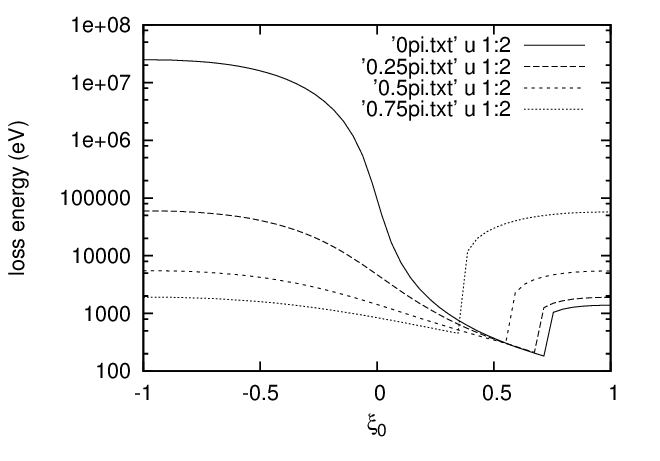
\includegraphics{/home/yj/project_new/pic_full-f/fig1/a.eps}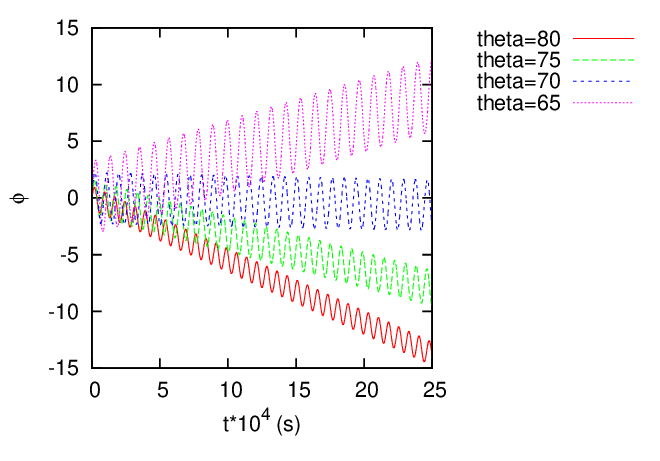
\includegraphics{/home/yj/project_new/pic_full-f/fig1/p2.eps}
  \caption{\label{12-20-e1}Electron distribution function in the phase-space
  evaluated at $t = 0$ and $\overline{t} = 17.5$ for a one-dimensional
  electrostatic simulation of the two-stream instability performed with
  $N_{\tmop{loaded}} = 2 \times 10^4$, $N = 1024$, $L / \lambda_D = 100$, $v_b
  / v_t = 3$, and $\delta t \omega_p = 0.1$.}
\end{figure}

to be continued.

My Fortran code solving the two-stream instability problem is in the directory
/home/yj/project\_new/pic\_full-f/ of my computer.

\section{Summary}

In summary, PIC = random sample of \ phase space (Monte-Carlo integration) +
particle spatial shape + field solver + characteristics (particle orbits)
and/or marker's weight integrator.

\section{\label{10-11-e1}Random number}

\subsection{Uniformly distributed random number}

Generating random numbers that are uniform distributed in the range $[0, 1]$
is the basis for generating non-uniform distribution. Because the same program
with the same input always produces the same output, it is not possible to
write a program that produces truly random numbers. However, for most
purposes, a pseudo-random number sequence will work almost as well. By
``pseudo-random number'', we mean a repeatable sequence of numbers that has
statistical properties similar to a random sequence. The most well-known
algorithm for generating pseudo-random sequences of integers is the linear
congruental method{\cite{Fitzpatrickcp}}, in which the $n$th and $(n + 1)$th
integers in the sequence is related by
\begin{equation}
  \label{2-19-e1} I_{n + 1} = \tmop{Mod} (A I_n + C, M),
\end{equation}
where $\tmop{Mod}$ is the remainder function, $A$, $C$, and $M$ are positive
integer constants. The first number in the sequence, which is called the seed
value, is selected by users. Equation (\ref{2-19-e1}) can generate
pseudo-random number that is uniform distributed in the range $[0, M - 1]$.
The obtained sequence can be scaled by a factor of $M - 1$ to lie in the range
$[0, 1]$. Figure \ref{7-9-p1} plots the possibility density of $10^6$ values
returned by Eq. (\ref{2-19-e1}) \ with parameters $A = 16807$, $C = 0$, $M =
2147483647$ (this choice is called the Park and Miller method). In practice we
need to use Schrange's algorithm to avoid integer
overflow{\cite{Fitzpatrickcp}}.

\begin{figure}[h]
  \includegraphics{/home/yj/project_new/pic_code/fig2/tmp.eps}
  \caption{\label{7-9-p1}The distribution of the $10^6$ values returned by the
  the random number generator Eq. (\ref{2-19-e1}). The possibility density
  (value of the distribution function) is obtained by the following steps: (1)
  divide the range $[0, 1]$ into 100 sub-regions; (2) then counts respectively
  the number of the returned value whose values are in the sub-regions; (3)
  the numbers of value in each sub-region obtained this way is further divided
  by the total number of values ($10^6$) to give the relativistic
  possibilities; (4) scale the relativistic possibilities by $100$ times,
  which gives the exact possibility density (this scaling is needed because
  the sub-region is of length $1 / 10$0, instead of unit length). Note that
  the value of the possibility density can be larger than one.}
\end{figure}

\

Another way to visualize whether the values generated by the random generator
are random distributed in the region $[0, 1]$ is to view how the points $(x_j,
x_{j + 1})$ are distributed in the two-dimension plane, as is plotted in Fig.
\ref{1-22-1}.

\begin{figure}[h]
  \includegraphics{/home/yj/project_new/pic_code/fig3/tmp.eps}
  \caption{\label{1-22-1}Plot of $x_j$ verse $x_{j + 1}$ for $j = 1, 2,
  \ldots, 10^4$. Here $x_j$ are random numbers generated by the random number
  generator.}
\end{figure}

\subsection{Non-uniformly distributed random number}

Consider the problem of generating random numbers that are distributed
according to some kind of non-uniform distribution function. There are two
methods of generating non-uniformly distributed random numbers satisfying a
given distribution function, namely, the transformation method and the
rejection method{\cite{Fitzpatrickcp}}. Let us examine these two methods in
turn.

\subsubsection{Transformation method}

Suppose there are two random variables $y$ and $x$ that are related to each
other by $y = f (x)$. If the probability density of $x$, $P_x (x)$, is known,
how do we calculate the probability of the random variable $y$? Using the
probability conservation, i.e,
\begin{equation}
  P_y (y) |d y| = P_x (x) |d x|,
\end{equation}
we obtain
\begin{equation}
  \label{11-5-1} P_y (y) = \frac{P_x (x)}{|f' (x) |},
\end{equation}
which gives the relation between $P_y (y)$ and $P (x)$. Next, consider the
inverse problem of the above, i.e., if we want to generate non-uniform
distribute random numbers $y$ with probability density being $P_y (y)$ from a
uniformly distributed random variables $x$, how do we choose the function $f
(x)$? In this case, $P (x) = 1$ and Eq. (\ref{11-5-1}) is written
\begin{equation}
  \label{11-5-2} P_y (f (x)) = \frac{1}{|f' (x) |},
\end{equation}
which can be solved to give $f (x)$. For a general function $P_y (y)$, Eq.
(\ref{11-5-2}) can not be solved analytically. For the special case $P_y (y) =
e^{- y}$ (Poisson distribution), we find that $f (x) = - \ln x$ solves Eq.
(\ref{11-5-2}). Therefore, we can generate Poisson distribution by the
following Fortran codes:
\begin{tmcode}
call random_number(x) !generate uniformly distributed random numbers in [0:1]
y=-log(x)
\end{tmcode}
The transformation method requires differential function $f (x)$ be known,
which is not always practical for a general probability density $P_y (y)$. In
such cases, we can use the rejection method discussed next.

\subsubsection{Rejection method}

Suppose that we want to generate non-uniformly distributed random numbers
between $x_{\min}$ and $x_{\max}$ that satisfy a given probability density $P
(x)$. To achieve this, we first generate a uniform random number $x_t$ between
$x_{\min}$ and $x_{\max}$. Then we generate another uniform random number $y$
between 0 and $P_{\max}$, where $P_{\max}$ are the maximal values of $P (x)$
for $x \in [x_{\min}, x_{\max}]$. If $P (x_t) > y$ then, $x_t$ is kept as a
desired random number, otherwise $x_t$ is discarded. Repeat this process, then
all the random numbers kept will satisfy the probability density $P (x)$ (need
thinking why, to be proved). This method is called the rejection method. It is
obvious how the rejection method generalizes to multiple-dimensional cases.

\subsubsection{Numerical examples}

The one-dimensional Gaussian distribution is given by
\begin{equation}
  \label{2-19-p1} P (y) = \frac{1}{\sqrt{2 \pi} \sigma} \exp \left( - \frac{(y
  - \overline{y})^2}{2 \sigma^2} \right) .
\end{equation}
Figure \ref{1-22-3} compares the possibility density of the $10^6$ numbers
generated by the numerical code with that of the analytic form in Eq.
(\ref{2-19-p1}), which indicates that the numerical result agrees well with
the analytic one.

\

\begin{figure}[h]
  \includegraphics{/home/yj/project_new/pic_code/fig1/tmp.eps}
  \caption{\label{1-22-3}The distribution of the $10^6$ values returned by the
  the Gaussian distribution generator (using the rejection method) with the
  parameters $\overline{y} = 5.0$ and $\sigma = 1.25$. The possibility density
  (value of the distribution function) is obtained as follows: (1) divide the
  range $[0, 10]$ into 100 sub-regions (2) then counts respectively the number
  of the returned value whose values are in the sub-regions (3) the numbers of
  value in each sub-region obtained this way is further divided by the total
  number of values ($10^6$) to give the relativistic possibilities. (4) scale
  the relativistic possibilities by $10$ times, which gives the exact
  possibility density (this scaling is needed because the sub-region is of
  length $1 / 10$, instead of unit length). The solid line in the figure is
  the value obtained by evaluating Eq. (\ref{2-19-p1}). The results indicates
  that the distribution returned by the Gaussian generator agrees well with
  the desired theoretic one.}
\end{figure}

\

Figure \ref{1-22-4} is a plot of $x_j$ verse $x_{j + 1}$ for $j = 1, 2,
\ldots, 10^4$, which shows how the points $(x_j, x_{j + 1})$ are distributed
in the two-dimension plane.

\begin{figure}[h]
  \includegraphics{/home/yj/project_new/pic_code/fig4/tmp.eps}
  \caption{\label{1-22-4}Plot of $x_j$ verse $x_{j + 1}$ for $j = 1, 2,
  \ldots, 10^4$. Here $x_j$ are random numbers generated by the Gaussian
  distribution generator.}
\end{figure}

\

\

\

\section{On the noise of PIC simulation}

My comments on the accuracy of the PIC method: The PIC method is more accurate
than the semi-Lagrangian continuous method because the PIC method uses the
Monte-Carlo method to evaluate the high-dimension phase-space integral, which
is more accurate than the corresponding methods used in the semi-Lagrangian
algorithm, which uses traditional regular-grids based methods to evaluate the
phase space integral.

**wrong or unclear**Because of the discrete representation of continuous media
(a marker representing many physical particles), the PIC method usually gives
rise to considerable fluctuations in the solution**. At present, I do not
fully understand why PIC approach gives rise to numerical noise while the
continuum approach does not seem to have this problem.==>Update: I think now I
understand the reason: The fluctuation in the number of sampling points per
spatial cell gives rise to the noise in the results. However, this noisy
result is not \ necessarily less accurate than a smooth result (a bigger error
may be hidden in a smooth result).

\subsection{Choices of sampling probability function}

The probability density function used in making the phase-space sampling can
be any reasonable function, which can be chosen to obtain desired resolution
of the phase-space. The most intuitive way of sampling the phase-space is to
sample it using the uniform probability density function, i.e., $p
(\mathbf{Z}) = 1 / V$, where $V$ is the total volume of the phase space.
Another frequently used sampling scheme is to load particle markers according
to the initial total distribution function of the physical particles. In this
case $P (\mathbf{Z}) = f_{\tmop{tot}} (\mathbf{Z}) / N_s$, where $N_s$ is the
total number of physical particles, i.e., $\int_V f_{\tmop{tot}} (\mathbf{Z})
d \Gamma = N_s$. (The method of generating random markers that satisfies a
given probability density function is discussed in Sec. \ref{10-11-e1}.)

\section{Finite element theory of particle-in-cell method}

Because of the use of finite-size shape, PIC method can also be considered as
a kind of finite element method{\cite{lapenta_pic}}.

\subsection{Finite element expansion of distribution function}

\begin{equation}
  f = \sum_p f_p (x, v, t)
\end{equation}
\begin{equation}
  f_p (x, v, t) = N_p S_x (x - x_p) S_v (v - v_p)
\end{equation}
where $N_p$, $x_p$, and $v_p$ are functions of only time $t$ and are
independent of $x$ and $v$.

\subsection{Basis functions: particle shape }

\

\

\subsection{Moment equations}

\


\begin{equation}
  \frac{\partial f}{\partial t} + v \frac{\partial f}{\partial x} +
  \frac{q_s}{m_s} E \frac{\partial f}{\partial v} = 0,
\end{equation}
\begin{equation}
  \sum_p \left( \frac{\partial N_p S_x (x - x_p) S_v (v - v_p)}{\partial t} +
  v \frac{\partial N_p S_x (x - x_p) S_v (v - v_p)}{\partial x} +
  \frac{q_s}{m_s} E \frac{\partial N_p S_x (x - x_p) S_v (v - v_p)}{\partial
  v} \right) = 0,
\end{equation}


\

---tmp--
\begin{equation}
  f = f_0 + \delta f
\end{equation}
\begin{equation}
  \frac{d \delta f}{d t} = - \frac{d f_0}{d t}
\end{equation}
\begin{equation}
  \frac{d \delta f / f}{d t} = - \frac{1}{f}  \frac{d f_0}{d t}
\end{equation}
\begin{equation}
  \frac{d \delta f / f}{d t} = - \frac{f_0}{f}  \frac{1}{f_0}  \frac{d f_0}{d
  t}
\end{equation}

\begin{equation}
  \frac{d w}{d t} = - \frac{f - \delta f}{f}  \frac{1}{f_0}  \frac{d f_0}{d t}
\end{equation}
\begin{equation}
  \frac{d w}{d t} = - (1 - w)  \frac{1}{f_0}  \frac{d f_0}{d t}
\end{equation}
to be deleted--

\

\

\

\appendix\section{From discrete microscopic distribution function to
statistic (continuum) distribution function}

A plasma can be considered to be composed of a set of classical point
particles, with motion subject to Newton's equations and with the Lorentz
forces and electromagnetic field derived from Maxwell's equations. Because of
the huge number of particles in a plasma, the above microscopic representation
is intractable, and simplifications must be sought{\cite{turner2006}}.

A usual procedure is to approximate the set of particles by a continuum
distribution function. This step involves some kind of averaging procedure to
remove certain spatial and temporal frequencies that are associated with the
graininess of the particle description (particle corelations, i.e.,
collisions). It is important to note that approximation is introduced in
passing from the microscopic particle representation to the continuum
distribution function.

The averaging procedure involves a small parameter, the so-called ``plasma
parameter,'' which is the inverse of the number of particles contained in a
Debye sphere. The collisionless Boltzmann equation, also known as the Vlasov
equation, emerges from the averaging procedure as the approximation at zero
order in the plasma parameter. What is discarded in the the zeroth order
approximation is the so-called collisional effects. In the first order
approximation, there appear additional terms, which is a representation of the
Coulomb collision effects.

The discrete microscopic distribution function (Klimontovich-Dupree
distribution function) (Chapter 3 in Nicholson (1983)) is written as
\begin{equation}
  F^M_{\alpha} (\mathbf{x}, \mathbf{v}, t) = \sum_{p_{\alpha} =
  1}^{N_{\alpha}} \delta_x^3 (\mathbf{x}-\mathbf{x}_{p_a}) \delta^3_v
  (\mathbf{v}-\mathbf{v}_{p_{\alpha}}) .
\end{equation}


Then the partial time derivative of $F_{\alpha}^M$ is written as
\begin{eqnarray}
  \frac{\partial F^M_{\alpha} (\mathbf{x}, \mathbf{v}, t)}{\partial t} & = &
  \sum_{p_{\alpha} = 1}^{N_{\alpha}} \delta^3_v
  (\mathbf{v}-\mathbf{v}_{p_{\alpha}}) \frac{\partial}{\partial t} \delta_x^3
  (\mathbf{x}-\mathbf{x}_{p_a}) + \sum_{p_{\alpha} = 1}^{N_{\alpha}}
  \delta_x^3 (\mathbf{x}-\mathbf{x}_{p_a}) \frac{\partial}{\partial t}
  \delta^3_v (\mathbf{v}-\mathbf{v}_{p_{\alpha}}) \\
  & = & - \sum_{p_{\alpha} = 1}^{N_{\alpha}} \delta^3_v
  (\mathbf{v}-\mathbf{v}_{p_{\alpha}}) \frac{\partial
  \mathbf{x}_{p_{\alpha}}}{\partial t} \cdot \nabla_{\mathbf{x}} [\delta_x^3
  (\mathbf{x}-\mathbf{x}_{p_a})] - \sum_{p_{\alpha} = 1}^{N_{\alpha}}
  \delta_x^3 (\mathbf{x}-\mathbf{x}_{p_a}) \frac{\partial
  \mathbf{v}_{p_{\alpha}}}{\partial t} \cdot \nabla_{\mathbf{v}} \delta^3_v
  (\mathbf{v}-\mathbf{v}_{p_{\alpha}}) \nonumber\\
  & = & - \sum_{p_{\alpha} = 1}^{N_{\alpha}} \delta^3_v
  (\mathbf{v}-\mathbf{v}_{p_{\alpha}}) \mathbf{v}_{p_{\alpha}} \cdot
  \nabla_{\mathbf{x}} [\delta_x^3 (\mathbf{x}-\mathbf{x}_{p_a})] -
  \sum_{p_{\alpha} = 1}^{N_{\alpha}} \delta_x^3 (\mathbf{x}-\mathbf{x}_{p_a})
  \frac{q_{\alpha}}{m_{\alpha}} [\mathbf{E}^M (\mathbf{x}_{p_{\alpha}})
  +\mathbf{v}_{p_{\alpha}} \times \mathbf{B}^M (\mathbf{x}_{p_{\alpha}})]
  \cdot \nabla_{\mathbf{v}} \delta^3_v (\mathbf{v}-\mathbf{v}_{p_{\alpha}}) 
  \label{18-12-14-p1}
\end{eqnarray}
Using the property of the Dirac delta function:


\begin{equation}
  a \delta (a - b) = b \delta (a - b)
\end{equation}
expression (\ref{18-12-14-p1}) is written as
\begin{eqnarray}
  \frac{\partial F^M_{\alpha} (\mathbf{x}, \mathbf{v}, t)}{\partial t} & = & -
  \sum_{p_{\alpha} = 1}^{N_{\alpha}} \delta^3_v
  (\mathbf{v}-\mathbf{v}_{p_{\alpha}}) \mathbf{v} \cdot \nabla_{\mathbf{x}}
  [\delta_x^3 (\mathbf{x}-\mathbf{x}_{p_a})] - \sum_{p_{\alpha} =
  1}^{N_{\alpha}} \delta_x^3 (\mathbf{x}-\mathbf{x}_{p_a})
  \frac{q_{\alpha}}{m_{\alpha}} [\mathbf{E}^M (\mathbf{x}) +\mathbf{v} \times
  \mathbf{B}^M (\mathbf{x})] \cdot \nabla_{\mathbf{v}} \delta^3_v
  (\mathbf{v}-\mathbf{v}_{p_{\alpha}}) \nonumber\\
  & = & -\mathbf{v} \cdot \nabla_{\mathbf{x}} \sum_{p_{\alpha} =
  1}^{N_{\alpha}} \delta^3_v (\mathbf{v}-\mathbf{v}_{p_{\alpha}}) [\delta_x^3
  (\mathbf{x}-\mathbf{x}_{p_a})] - \frac{q_{\alpha}}{m_{\alpha}} [\mathbf{E}^M
  (\mathbf{x}) +\mathbf{v} \times \mathbf{B}^M (\mathbf{x})] \cdot
  \nabla_{\mathbf{v}} \sum_{p_{\alpha} = 1}^{N_{\alpha}} \delta_x^3
  (\mathbf{x}-\mathbf{x}_{p_a}) \delta^3_v
  (\mathbf{v}-\mathbf{v}_{p_{\alpha}}) \nonumber\\
  & = & -\mathbf{v} \cdot F_{\alpha}^M - \frac{q_{\alpha}}{m_{\alpha}}
  [\mathbf{E}^M (\mathbf{x}) +\mathbf{v} \times \mathbf{B}^M (\mathbf{x})]
  \cdot \nabla_{\mathbf{v}} F_{\alpha}^M, 
\end{eqnarray}
i.e.,
\begin{equation}
  \frac{\partial F^M_{\alpha} (\mathbf{x}, \mathbf{v}, t)}{\partial t}
  +\mathbf{v} \cdot F_{\alpha}^M + \frac{q_{\alpha}}{m_{\alpha}} [\mathbf{E}^M
  (\mathbf{x}) +\mathbf{v} \times \mathbf{B}^M (\mathbf{x})] \cdot
  \nabla_{\mathbf{v}} F_{\alpha}^M = 0
\end{equation}
This is the Klimontovich equation of the microscopic distribution function.

\

Note that Boltzmann equation provide a mesoscopic rather than a microscopic
description because of the spatio-temporal averaging involved in deriving the
Boltzmann equation

The particle-in-cell (PIC) method has obvious structural similarities to a
direct simulation of the microscopic model of the plasma outlined above, but
this is essentially misleading: Particle-in-cell simulation should be
understood to be a Monte Carlo solution of the Boltzmann equation (or the
Vlasov equation), i.e., the PIC method is solving a continuum mesoscopic
kinetic equation rather than the primitive microscopic model of a plasma.

\

two things that reduce collision: (1) finite-size particle used in doing the
deposition and force iterpolation and (2) finite grid size used in solving the
field equation.

The nearest grid point deposition and force interpolation correspond zero
sized particle, i.e., delta function
\begin{equation}
  S (x) = \frac{1}{\Delta x} \delta \left( \frac{x}{\Delta x} \right) .
\end{equation}


\begin{thebibliography}{1}
  \bibitem[1]{allfrey2003}S.J. Allfrey and R.~Hatzky. {\newblock}A revised
  delta-f algorithm for nonlinear pic simulation.
  {\newblock}\tmtextit{Computer Physics Communications}, 154(2):98 -- 104,
  2003.
  
  \bibitem[2]{aydemir1994}A.~Y. Aydemir. {\newblock}A unified monte carlo
  interpretation of particle simulations and applications to non-neutral
  plasmas. {\newblock}\tmtextit{Physics of Plasmas}, 1(4):822--831, 1994.
  
  \bibitem[3]{chen1997}Yang Chen and Roscoe~B. White. {\newblock}Collisional
  delta-f method. {\newblock}\tmtextit{Physics of Plasmas}, 4(10):3591--3598,
  1997.
  
  \bibitem[4]{Fitzpatrickcp}Richard Fitzpatrick.
  {\newblock}\tmtextit{Computational Physics:An introductory course}.
  {\newblock}Richard Fitzpatrick, 2004.
  
  \bibitem[5]{gurnett2004}D.~A. Gurnett and A.~Bhattacharjee.
  {\newblock}\tmtextit{Introduction to plasma physics : with space and
  laboratory applications}. {\newblock}Cambridge University Press, Cambridge,
  UK, 2004.
  
  \bibitem[6]{artcompsci}Piet Hut and Jun Makino.
  {\newblock}\tmtextit{http://www.artcompsci.org/vol\tmrsub{1}/v1\tmrsub{w}eb/node34.html}.
  {\newblock}Online, 2012.
  
  \bibitem[7]{lapenta_pic}Giovanni Lapenta. {\newblock}\tmtextit{Particle In
  Cell Methods With Application to Simulations in Space Weather}.
  {\newblock}Online, 2012.
  
  \bibitem[8]{turner2006}M.~M. Turner. {\newblock}Kinetic properties of
  particle-in-cell simulations compromised by monte carlo collisions.
  {\newblock}\tmtextit{Physics of Plasmas}, 13(3):033506, 2006.
\end{thebibliography}

\

\

\

\

\

\

\

\

\

\

\end{document}
